% Created 2017-11-23 Thu 19:28
% Intended LaTeX compiler: pdflatex
\documentclass[11pt]{article}
\usepackage[utf8]{inputenc}
\usepackage[T1]{fontenc}
\usepackage{graphicx}
\usepackage{grffile}
\usepackage{longtable}
\usepackage{wrapfig}
\usepackage{rotating}
\usepackage[normalem]{ulem}
\usepackage{amsmath}
\usepackage{textcomp}
\usepackage{amssymb}
\usepackage{capt-of}
\usepackage{hyperref}
\usepackage{wasysym,bussproofs}
\date{\today}
\title{}
\hypersetup{
 pdfauthor={},
 pdftitle={},
 pdfkeywords={},
 pdfsubject={},
 pdfcreator={Emacs 25.3.1 (Org mode 9.1.2)}, 
 pdflang={English}}
\begin{document}

\tableofcontents

\section{Lecture 1 \textit{<2017-09-05 Tue>}}
\label{sec:orgd22cd7a}
Logic \& Computability
Prof. Dirk Schlimm
\begin{itemize}
\item Find out what Schlimm means for the next lecture
\item Great for people in computer science, but everyone else too
\begin{itemize}
\item Essential material that everyone should know
\item Stable material, as the material is old
\item Very abstract and technical material, even if it does not require a solid mathematical background
\item \uline{Hard} course
\begin{itemize}
\item Important to give feedback to the professor
\end{itemize}
\end{itemize}
\end{itemize}
This course complements the textbook, Godel, Escher Bach.

\subsection{Homework}
\label{sec:org69cd79f}
is not graded, just checked if done.
\begin{itemize}
\item Why?
\begin{itemize}
\item To motivate us to do homework exercises
\item Practice is important, the course is hard
\item TAs don't need to correct them, so they can hold more office hours
\end{itemize}
\end{itemize}

Discussion board on MyCourses. Do not email the professor, ask questions on discussion board so everyone can see the answer (incase they have the same question).

Some times there will be intentional mistakes on the board.
\begin{itemize}
\item To make it easier to ask questions
\item To motivate us to pay attention
\end{itemize}

There are no stupid questions, even if you ask the same question as the person before you. Perhaps the professor's answer was unclear.
The most stupid question is the one not being asked.
\subsection{Quizzes}
\label{sec:orge692a37}
\begin{itemize}
\item 3 quizzes throughout this course
\item Dates will be on the schedule on professor's website
\item In class, 15-20 minutes long
\item Each one is graded and worth 10\%
\item Fairly straightforward, some are even definitions
\item To make sure you've done your work
\end{itemize}

Midterm is 25\%, Final is 40\%

\subsection{Proofs}
\label{sec:orgafa6e0f}
We will see lots of proofs, different kinds of proofs.
\begin{itemize}
\item Direct: Go from assumption towards the theorem
\item Indirect: Negation of claim \(\rightarrow\) contradiction \(\rightarrow\) claim
\begin{itemize}
\item Sometimes called proof by contradiction
\end{itemize}
\item Biconditional: \(2\) claims, \(p,q\)
\begin{itemize}
\item Start with \(p\) and prove \(q\) but also start with \(q\) and prove \(p\)
\end{itemize}
\item By cases: Split claim into several cases
\begin{itemize}
\item case 1, case 2, case 3
\item Each one proves the same conclusion
\item If the cases were exhaustive, then you have proved the claim
\end{itemize}
\item Induction (to be taught next lecture)
\end{itemize}

So you can split a proof into subproofs of these kinds.

\subsubsection{Example Proofs}
\label{sec:orgc21cd19}
\begin{enumerate}
\item Thm
\label{sec:org3fc06d2}
\(\sqrt{2}\) is nor rational.
\begin{itemize}
\item Rational: Fractions: \(\frac{x}{y}\)
\end{itemize}
If you have a square with sides of length 1, the length of the diagonal is \(\sqrt{2}\)
Pythagoras proved this.
\begin{enumerate}
\item Def 1
\label{sec:orgd2fbc7e}
A natural number \(a\) is \uline{even} if and only if (iff) \(\exists\) a natural number \(b\), such that \(a=2b\).
\item Lemma 1
\label{sec:org4e5bc78}
For any number \(a\), \(a^2\) is even \uline{iff} \(a\) is even.
\begin{itemize}
\item Biconditional, since iff
\end{itemize}
\begin{enumerate}
\item Proof:
\label{sec:orgcf02908}
\(\leftarrow\) Assume: \uline{\(a\) is even}.
So there is: \(a=2b\) (by def. 1)

\(a^2=(2b)^=4b^2=2(\underbrace{2b^2}_c)\) (square)
So, \uline{\(a^2\) is even}, since it is \(2\) times \(c\), a natural number.

\(\rightarrow\) (DIY)
Assume: \uline{\(a^2\) is even}.
So there is: \(a^2=2b\) (by def. 1)
\end{enumerate}

\item Lemma 2
\label{sec:orgc97eb12}
For any rational number \(x\), there are natural numbers \(a\) and \(b\), \uline{not both even}, s.t. \(x=\frac{a}{b}\)
\begin{itemize}
\item If they were both even, you could simplify the fraction by dividing by 2.
\end{itemize}
Proof omitted for this lemma.
\item Proof of Thm:
\label{sec:org76a9b4a}
Indirect proof. (Contradiction)
Assume (for reductio/contradiction): \(\sqrt{2}\) is rational.
By Lemma 2, \(\exists\) natural numbers \uline{\(a\) and \(b\) not both even} s.t. \(\sqrt{2}=\frac{a}{b}\)

Square: \(2=\left(\frac{a}{b}\right)^2=\frac{a^2}{b^2}\)
\(a^2=2b^2\)

So \(a^2\) is even (by def. 1)
\uline{\(a\) is even} by (lemma 1)
If \(a\) is even, we can write: \(a=2c\) (by def 1)
Square: \(a^2=(2c)^2=4c^2=a^2\)

\(4c^2=2b^2\)

Divide by 2: \(2c^2=b^2\)
So \(b^2\) is even (def. 1)
\uline{\(b\) is even} (by lemma 1)

Contradiction! Assumption is false, therefore \(\sqrt{2}\) is \uline{not} rational. \(\Box\)
\end{enumerate}
\item {\bfseries\sffamily TODO} Download Handout and read it
\label{sec:org2c764c2}
\end{enumerate}
\section{Lecture 2 \textit{<2017-09-07 Thu>}}
\label{sec:org69a35a1}
Last class we talked about proofs \& types of proofs.
Next week we'll be talking about sets and countability and comparing them all. Will talk about density of rationals and irrationals, to say which is bigger.
\subsection{Things that are infinite}
\label{sec:org7e5ee70}
\begin{itemize}
\item Natural numbers
\item Rational numbers
\item Infinite lists
\end{itemize}
\begin{enumerate}
\item How do you prove things about infinitely large things?
\label{sec:orge59c2a1}
\begin{itemize}
\item Counter example
\begin{itemize}
\item All swans are white
\begin{itemize}
\item Show one that isn't white
\end{itemize}
\end{itemize}
\item Pick an arbitrary example and show that it works for that
\begin{itemize}
\item Use particular properties about an arbitrary object to show that something works for all of them
\end{itemize}
\end{itemize}
\end{enumerate}
\subsection{Mathematical induction}
\label{sec:org8f810e0}
\begin{itemize}
\item Inference (step):
\begin{itemize}
\item Certain number of assumptions/premises \(A_n\ldots A_n\)
\item Conclusion
\end{itemize}
\end{itemize}
\subsubsection{Deduction:}
\label{sec:org8bee806}
\begin{itemize}
\item It is impossible for the premises of an inference step to be \uline{true} and the conclusion \uline{false}.
\item The conclusion follows \uline{necessarily} from the premises. (reformulation of above)
\end{itemize}
\begin{enumerate}
\item e.g.
\label{sec:orgcfe9759}
\(\frac{\text{if }A \text{ then }B \hspace{5 pt}A}{B}\)
\begin{itemize}
\item MODUS PONENS (type of deductive inference)
\end{itemize}
\end{enumerate}
\subsubsection{Induction:}
\label{sec:orgd00776f}
\begin{itemize}
\item The premises make the conclusion \uline{more likely}
\item My cat is smart, my friend's cat is smart, my parent's cat is smart, so all cats are smart
\begin{itemize}
\item Inductive argument, makes it more likely, but doesn't see them all
\end{itemize}
\end{itemize}
\subsubsection{Inductive or Deductive?}
\label{sec:org82753dc}
\begin{enumerate}
\item Claim
\label{sec:org156dcd9}
Let \(n\) be the number of points on a circle. Then the number of regions obtained by pairwise connecting each point is \(R=2^{n-1}\)
\begin{enumerate}
\item Argument
\label{sec:org2e2a8a3}
\begin{center}
\begin{tabular}{ll}
\(n\) & \(R\)\\
\hline
\(1\) & \(1=2^0\)\\
\(2\) & \(2=2^1\)\\
\(3\) & \(4=2^2\)\\
\(4\) & \(8=2^3\)\\
\(5\) & \(16=2^4\)\\
\(6\) & \(31\)\\
\end{tabular}
\end{center}

\begin{center}
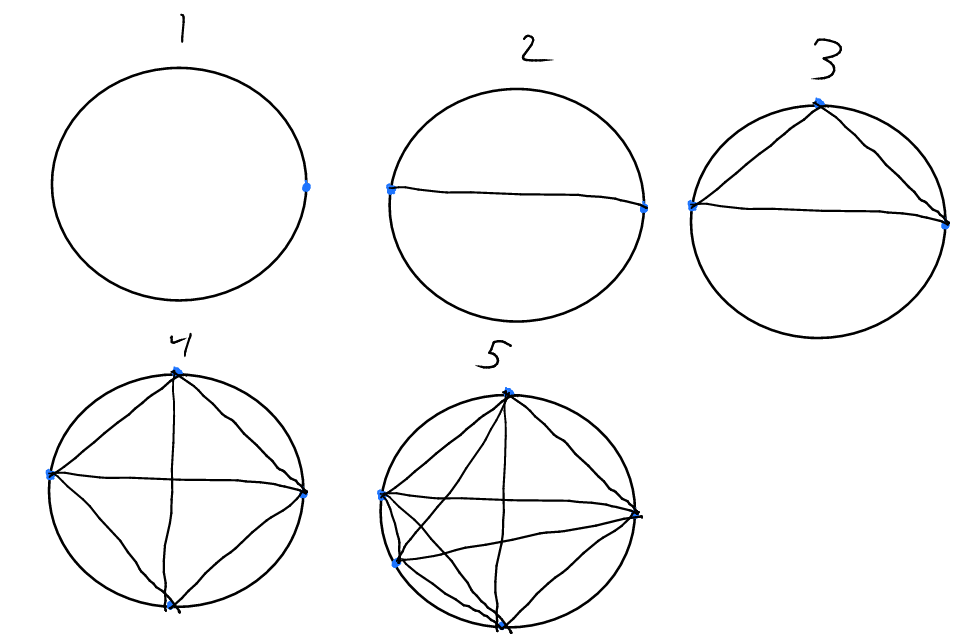
\includegraphics[width=.9\linewidth]{./Images/i1.png}
\end{center}   

\begin{itemize}
\item Inductive argument
\item What was wrong with the argument?
\begin{itemize}
\item We saw a pattern, but\ldots{}
\begin{itemize}
\item There's no reason for the jump from each \(n\) to have something in common
\item If they had something in common, then it would continue holding for the next one
\end{itemize}
\item Therefore induction makes the premise more likely
\begin{itemize}
\item But does not establish it deductively
\end{itemize}
\item So in order to rigorously prove something inductively, we need mathematical induction
\end{itemize}
\end{itemize}
\end{enumerate}
\end{enumerate}

\subsection{Handout}
\label{sec:org3ade0bb}
\subsubsection{Recursive (inductive) definition:}
\label{sec:org4ddd0e4}
\begin{enumerate}
\item Base clause(s) defines basic elements.
\item Inductive clause(s): How to build up complex elements from parts
\item Final clause: Nothing else is an element (bookkeeping)
\end{enumerate}
\begin{enumerate}
\item E.g.
\label{sec:orgf154807}
\begin{enumerate}
\item \(\mathbb{N}\)
\begin{itemize}
\item Base clause \(0\) is in \(\mathbb{N}\)
\item Inductive clause: if \(x \in \mathbb{N}\) then \(s(x)\) (successor of \(x\)) then \(s(x)\) is in \(\mathbb{N}\)
\item Final clause: Nothing else is in \(\mathbb{N}\)
\item So natural numbers are:
\begin{itemize}
\item \(0, s(0), s(s(0)), \ldots\)
\end{itemize}
\end{itemize}
\item Even numbers or odd numbers
\begin{itemize}
\item Take successor of successor, take \(0\) as base clause for even, \(1\) for odd
\end{itemize}
\item Lists
\begin{itemize}
\item Empty list is a list
\item What you get from adding to a list is also a list
\end{itemize}
\item Dominoes
\begin{itemize}
\item When you have a domino, you can place one 2 cm behind it
\item Push first one, they all fall
\begin{itemize}
\item To prove they all fall, have to show they all have a certain amount of space between them
\begin{itemize}
\item Relates to proof by mathematical induction
\end{itemize}
\end{itemize}
\end{itemize}
\end{enumerate}
\item Proof by mathematical induction
\label{sec:org8a94e48}
\begin{enumerate}
\item Base case: Show that the property holds of the basic elements.
\item Inductive step:
\begin{enumerate}
\item Assume that the property holds for some element \(n\) (Inductive Hypothesis)
\item \uline{Show}: holds for elements generated from \(n\) by inductive clauses.
\end{enumerate}
\item Conclusion: Property holds \uline{for all} elements.
\end{enumerate}
This is \textbf{deductive inference}!
What are the premises?
\begin{itemize}
\item For natural numbers:
\begin{itemize}
\item \(\frac{\overbrace{P(0)}^{\text{Base case}} \overbrace{P(n)}^{\text{IH}}\overbrace{\to}^{\text{Ind. step}} P(s(n))}{\forall x P(x)}\)
\end{itemize}
\end{itemize}
\item Variant (strong/complete induction):
\label{sec:org8fd0741}
\begin{itemize}
\item \uline{Ind. Step.}
\begin{enumerate}
\item Assume that \(P\) holds for all elements \uline{less than} \(n\)
\item Show: \(P\) holds of \(n\)
\end{enumerate}
\item \uline{No base case}
\item See example 5.5!
\end{itemize}
\end{enumerate}
\subsubsection{Theorem}
\label{sec:org7fcbe90}
For any nat. number \(n\geq 1\), the sum \(\underbrace{1+2+\ldots+n}_{\sum_i=1^n i}=\frac{n(n+1)}{2}\)
(If you do a proof for your homework or on an exam, always include many details. You can even use a template to structure your proofs the same way, useful for steps for induction.)
\begin{enumerate}
\item Proof (by math. ind)
\label{sec:orgf1f5d6f}
\begin{enumerate}
\item Base case: Show claim holds for \(n=1=\frac{1(1+1)}{2}\)
\item Ind. step.
\begin{enumerate}
\item I.H. The claim holds for \(m\): \(\sum_{i=1}^m i = \frac{m(m+1)}{2}\)
\item Show: The claim holds for \(m+1\)
\end{enumerate}
\end{enumerate}
2 strategies, either \(\frac{n(n+1)}{2}\to {1+2+\ldots+n}\) or \({1+2+\ldots+n}\to \frac{n(n+1)}{2}\). Will be doing 2nd.
\(1+2+\ldots+(m+1)=\sum_{i=1}^{m+1}i=\sum_{i=1}^m i + (m+1)\)

\(=\frac{m(m+1)}{2}+(m+1)\) (by I.H.)

\(=\frac{m(m+1)+2m+2}{2}=\frac{(m+1)(m+2)}{2}\)
\begin{enumerate}
\item Conclusion: The claim holds \uline{for all} \(n\geq 1\) \(\Box\)
\end{enumerate}
\end{enumerate}
\section{Lecture 3 \textit{<2017-09-12 Tue>}}
\label{sec:orga0bf96e}
\subsection{Set theory}
\label{sec:org383a3e2}
All that is being said here is taken from the reading mathematical introduction to logic chapter zero.

A \uline{set} is a thing with elements. We can present sets in two ways:
\begin{itemize}
\item Extensional:
\begin{itemize}
\item Presentation
\item \(\{1,2,3\}\)
\end{itemize}
\item Intensional:
\begin{itemize}
\item Given a set \(A\), and a property \(P\): \(\{x\in A|P(x)\}\)
\end{itemize}
\end{itemize}
\subsubsection{Ex}
\label{sec:orge386c95}
\(\mathbb{N}\): the set of natural numbers.

\(D=\{x\in \mathbb{N}|x \text{ is prime}\}=\{2,3,5,7,11, \ldots\}\)
\subsubsection{Definitions}
\label{sec:orga1131f8}
\begin{itemize}
\item \(A\subseteq B \iff \forall x, x\in A \implies x \in B\)
\item \(A=B \iff (A\subseteq B) \wedge (B\subseteq A)\)
\item \(A \underbrace{\subset}_{\text{Proper subset}} B \iff (A\subseteq B)\wedge (A\neq B)\)
\item Empty set: \(\emptyset, \{\}\)
\begin{itemize}
\item When is \(x\in \emptyset\)? Never.
\item \(\emptyset \subseteq X\)? Always.
\begin{itemize}
\item Since all elements of the empty set are in \(X\).
\end{itemize}
\item \(\emptyset \in X\)?. If \(X\) contains \(\emptyset\).
\begin{itemize}
\item E.g. \(X=\{\{\},4\}\)
\end{itemize}
\end{itemize}
\end{itemize}
\(A=\{2,4,8\}, B=\{a,4,z\}\)
\begin{itemize}
\item \(\underbrace{A\cap B}_{\text{intersection}}: \forall x, (x\in A) \wedge (x\in B)\)
\begin{itemize}
\item \(A\cap B = \{4\}\)
\end{itemize}
\item \(\underbrace{A\cup B}_{\text{union}}: \forall x, (x\in A) \vee (x\in B)\)
\begin{itemize}
\item \(A\cup B = \{2,4,8,a,z\}\)
\end{itemize}
\item complement: \(\bar{A}:\) all elements that are not in \(A\) (from the \uline{universe of discourse}, the universe we're talking about)
\item Power set \(\frak{P}(A):\) the set of all subsets of \(A\)
\begin{itemize}
\item E.g. \(\frak{P}(B)=\{\emptyset,\{a\},\{4\},\{z\},\{a,4\},\{a,z\},\{4,z\},\{a,4,z\}\}\)
\item If \(A\) has \(n\) elements, \(\frak{P}(A)\) has \(2^n\) elements.
\end{itemize}
\item Is \(\{\emptyset,a\}\subseteq\{a,4,z\}\)? No.
\end{itemize}
\subsection{Tuples:}
\label{sec:orgfe325b4}
Like sets, but order matters.
\begin{itemize}
\item Ordered pair: \(\langle a,b \rangle = \{\{a\},\{a,b\}\}\)
\item \(\langle a,4,z \rangle \neq \langle 4,a,z \rangle\)
\end{itemize}
\subsubsection{Cross-product}
\label{sec:orgf543592}
\(A \times B \iff \{\langle x,y \rangle|x \in A \wedge y\in B\}\)
\begin{itemize}
\item If \(A\) has \(n\) elements, \(B\) has \(m\) elements
\item then \(A \times B\) has \(n\cdot m\) elements
\item and there are \(2^{n \cdot m}\) relations between \(A\) and \(B\)
\begin{itemize}
\item Since this is essential just the cardinality of the power set of the cross product
\item E.g. \(n=5, m=5\). 2 pairs of 5 friends. How many relations are possible? \(2^{25}=33,554,432\)
\end{itemize}
\end{itemize}
\subsubsection{Relations}
\label{sec:orgc4c300d}
\begin{itemize}
\item \(A=\{\text{John, Paul, George}\}\)
\item \(B=\{\text{guitar, bass}\}\)
\item \(\{\langle \text{John, guitar}\rangle, \langle \text{Paul, bass} \rangle, \langle \text{George, guitar} \rangle\}=R_1\)
\item \(R_2 = \{\langle \text{John, bass} \rangle\}\)
\end{itemize}
A \uline{relation} \(R\) on \(A\) and \(B\) is a subset of \(A\times B\).
\begin{itemize}
\item Elements of relations are tuples.
\end{itemize}
\uline{Domain} of a relation \(R: \{a| \text{there is a b, s.t. }\langle a,b \rangle \in R\}\)
\begin{itemize}
\item domain of \(R_1: \{\text{John, Paul, George}\}\)
\item domain of \(R_2: \{\text{John}\}\)
\end{itemize}
\uline{Range} of a relation \(R\): \(\{b| \text{there is an a, s.t. } \langle a,b
 \rangle \in R\}\)
\begin{enumerate}
\item Functions
\label{sec:org7717439}
A total \uline{function} \(f:A\to B\) is a binary relation \(R\), on \(A\) and \(B\) such that.
\begin{itemize}
\item It is \uline{single-valued}
\begin{itemize}
\item Every element in \(A\) is mapped to exactly one element in \(B\)
\end{itemize}
\item The domain of \(R\) is \(A\)
\end{itemize}
\begin{center}
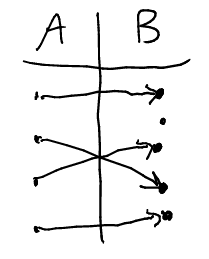
\includegraphics[width=.9\linewidth]{./Images/i2.png}
\end{center}
\begin{enumerate}
\item Definitions
\label{sec:org36a7d17}
\begin{itemize}
\item A function is \uline{injective} (one-to-one), if each element in the range is mapped to by exactly one element.
\begin{itemize}
\item To show this: Assume \(f(x)=f(y)\)
\begin{itemize}
\item Show \(x=y\)
\end{itemize}
\item So you don't have the situation that: \begin{center}
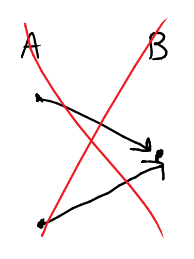
\includegraphics[width=.9\linewidth]{./Images/i3.png}
\end{center}
\end{itemize}
\end{itemize}

\begin{center}
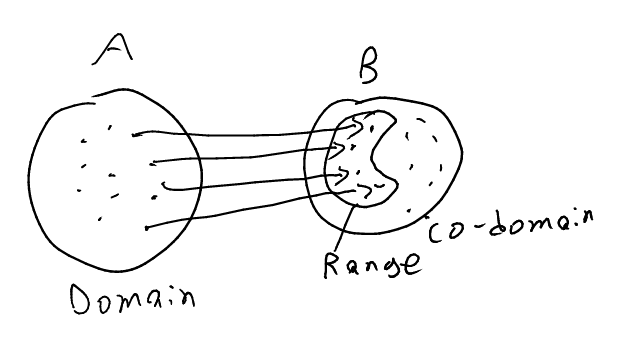
\includegraphics[width=.9\linewidth]{./Images/i4.png}
\end{center} 

\begin{itemize}
\item A function is \uline{surjective} if the \(range=codomain\).
\item A function that is both injective and surjective is \uline{bijective}.
\end{itemize}
\end{enumerate}
\end{enumerate}
\section{Lecture 4 \textit{<2017-09-14 Thu>}}
\label{sec:org364598e}
\subsection{Recap}
\label{sec:org04a66d7}
We talked about sets last class, such as:
\begin{itemize}
\item \(\{1,4,z\}\)
\item \(|\{1,4,z\}| = 3\) (Cardinality)
\end{itemize}

\noindent\rule{\textwidth}{0.5pt}
Are there more students or chairs in this class? 
\begin{itemize}
\item There are more chairs.
\item Matched students with chairs and to see what is left
\item f(students) \(\to\) chairs
\begin{itemize}
\item Injective function (can't have 2 students on one chair)
\item Every element of the range must be mapped to something
\item No element in the range can map to two elements
\end{itemize}
\item \(\implies |S| \leq |C| \iff\) there is an injective function from \(S\) to \(C\).
\end{itemize}

Cantor: \(|A|=|B| \iff |A| \leq |B|\) and \(|B|\leq |A| \iff\) there is a bijection between \(A\) and \(B\).
\subsection{More on sets}
\label{sec:org0ebbd05}
\subsubsection{Cardinalities}
\label{sec:orgc700a26}
A set D is \uline{finite} if its cardinality is a natural number.
\begin{itemize}
\item \(D \leftrightarrow \{1,\ldots,n\}\) (bijective function with natural numbers exists)
\end{itemize}
A set is \uline{countably infinite} (denumerable), if it is equinumerous to \(\mathbb{N}\) (bijection from this set to all the natural numbers).
\begin{itemize}
\item \(E=\{2,4,6,8,\ldots\}\)
\begin{itemize}
\item \(|E| = |\mathbb{N}| = |\mathbb{Z}|=|\mathbb{Q}|<|\mathbb{R}|\)
\end{itemize}
\end{itemize}
\begin{center}
\begin{tabular}{llllll}
\(\mathbb{N}\) & \(1\) & \(2\) & \(3\) & \(4\) & \ldots{} \(n\)\\
\hline
\(E\) & \(2\) & \(4\) & \(6\) & \(8\) & \ldots{}\(2n\)\\
\end{tabular}
\end{center}
\(f(x)=2x, \mathbb{N}\to E\)

\(\mathbb{Z}=\{\ldots -3, -2, -1, 0, 1, 2, 3, \ldots\}\)
\begin{itemize}
\item Is this bigger than the cardinality of the natural numbers?
\begin{itemize}
\item No, it's the same size, bijection. Even to positive, odds to negative.
\end{itemize}
\end{itemize}

\begin{center}
\begin{tabular}{lllllll}
\(-3\) & \(-2\) & \(-1\) & \(0\) & \(1\) & \(2\) & \(3\)\\
\hline
\(5\) & \(3\) & \(1\) & \(0\) & \(2\) & \(4\) & \(6\)\\
\end{tabular}
\end{center}

\(\mathbb{Q}^+ = \{\frac{x}{y}|x,y \in \mathbb{N}\}\)
\begin{itemize}
\item Are there more?
\end{itemize}
\begin{center}
\begin{tabular}{rlllllll}
 & 1 & 2 & 3 & 4 & 5 & 6 & \ldots{}\\
\hline
1 & 1/1 & 1/2 & 1/3 & 1/4 & 1/5 & 1/6 & \ldots{}\\
2 & 2/1 & 2/2 & 2/3 & 2/4 & 2/5 & 2/6 & \ldots{}\\
3 & 3/1 & 3/2 & 3/3 & 3/4 & 3/5 &  & \\
4 & 4/1 & 4/2 & 4/3 & 4/4 &  &  & \\
5 & 5/1 & 5/2 & 5/3 &  &  &  & \\
6 &  &  &  &  &  &  & \\
\end{tabular}
\end{center}
There are duplicates here though. So, instead of counting left to right, count diagonally.
\begin{itemize}
\item i.e. 1:1/1, 2:1/2, 3:2/1, 4:3/1, 5:2/2, 6:1/3, \ldots{}
\end{itemize}

\(\mathbb{R} = \mathbb{Q} \cup \{\text{irrationals}\}\)
\begin{itemize}
\item What are real numbers? All numbers that can be expressed via decimal expansion.
\item \(x.xxxxx\ldots\)
\item Is this countably infinite? No.
\end{itemize}
\subsubsection{Proof (by contradiction):}
\label{sec:orgbb7b86c}
Assume \(|\mathbb{N}|=|\mathbb{R}^{0.1}|\). 
(\(\mathbb{R}^{0.1} = \{x \in \mathbb{R}| 0<x<1\}\).)

Therefore, there is a bijection \(f: \mathbb{N} \to \mathbb{R}^{0.1}\)

Then, we can build the following table:
\begin{center}
\begin{tabular}{ll}
\(\mathbb{N}\) & \\
\hline
\(0\) & \(f(0)=0.12345\ldots\)\\
\(1\) & \(f(1)=0.33333\ldots\)\\
\(2\) & \(f(2)=0.5000 \ldots\)\\
\(3\) & \(f(3)=0.011101\ldots\)\\
\(4\) & \(\ldots\)\\
\(\ldots\) & \(\ldots\)\\
\(n\) & \(f(n)=0.112\ldots=z\)\\
\end{tabular}
\end{center}

Can you explain this table? Not really. Why?
\begin{itemize}
\item Construct new number \(z\):
\begin{itemize}
\item \(z=0.z_1z_2z_3z_4\ldots\)
\item Rule for constructing \(z\):
\end{itemize}
\end{itemize}
\begin{equation*}
z_i= \begin{cases}
1 & \text{if } f(i)_j \neq 1 \text{ where $f(i)_j$ is the ith digit in the decimal expansion of f(i)}
\\ 2 & \text{otherwise}
\end{cases}
\end{equation*}
\begin{itemize}
\item \(f(1)_1 = 3\)
\item \(f(2)_2 = 0\)
\item \(f(3)_3 = 1\)
\item \(\implies z=0.112\ldots\)
\item By construction, \(z\) is a real number between \(0\) and \(1\).
\item So it must be in the table, say in line \(n\).
\end{itemize}
What is \(z_n\)?
\begin{itemize}
\item Two cases:
\begin{itemize}
\item \(z_n = 2 = f(n)_n\) if \(f(n)_n = 1\) \lightning
\item \(z_n = 1 = f(n)_n\) if \(f(n)_n \neq 1\) \lightning
\item \(\implies\) contradiction!
\begin{itemize}
\item The assumption is false.
\end{itemize}
\end{itemize}
\end{itemize}
\section{Lecture 5 \textit{<2017-09-19 Tue>}}
\label{sec:org12c42a7}
\begin{itemize}
\item Quiz in one week
\item 20 minutes, in class
\item 8-10 questions, very simple
\begin{itemize}
\item Everything that was said in class
\item Everything done in the homework
\item Readings
\end{itemize}
\end{itemize}
\subsection{Recap}
\label{sec:orgb508df7}
Last class, we proved:
(Size of Natural numbers) \(\aleph_0 < |\mathbb{R}|\)
\(\implies\) Diagonalization
\begin{itemize}
\item We had a table and changed every element on the diagonal in order to get a new element
\item We will see many more proofs by diagonalization
\item Homework question: \(|\frak{P}(\mathbb{N})|>|\mathbb{N}|\)
\begin{itemize}
\item In general though, \(|\frak{P}(x)|>|x|\) (Cantor's theorem)
\begin{itemize}
\item What does this imply? There are infinite amount of infinite cardinalities (power set is bigger, power set of the power set is even bigger, \ldots{})
\item \(|\mathbb{N}|<|\frak{P}(\mathbb{N})|=|\mathbb{R}|=2^{\aleph_0}<|\frak{P}(\frak{P}(\mathbb{N}))|\)
\end{itemize}
\end{itemize}
\end{itemize}

\subsection{Cardinality}
\label{sec:org61324bc}
Things that have the same cardinality:
\subsubsection{Countable:}
\label{sec:org395dc4c}
\(|\mathbb{N}|\):
\begin{itemize}
\item E
\item \(\mathbb{Z}\)
\item \(\mathbb{Q}\)
\item English words
\item Sentences
\begin{itemize}
\item Finite objects that you can list
\item Why doesn't diagonalization work on sentences?
\end{itemize}
\item Programs
\item MIU strings
\item MIU theorems
\item If you can list them, they're countable
\end{itemize}
\subsubsection{Uncountable}
\label{sec:org03a0b76}
\(|\frak{P}(\mathbb{N})|\)
\begin{itemize}
\item \(\mathbb{C}\)
\item \(\mathbb{R}\)
\item Functions from \(\mathbb{N} \to \mathbb{N}\)
\begin{itemize}
\item From \(\mathbb{N} \to \{0,1\}\)
\end{itemize}
\end{itemize}

\noindent\rule{\textwidth}{0.5pt}
\subsection{Formal Systems (GEB CH. 1)}
\label{sec:orgc8efbfe}
\subsubsection{Examples}
\label{sec:orgaf1f790}
\begin{itemize}
\item Programming languages
\item Logic
\item Computation: TM
\item Formal arithmetic
\end{itemize}

\noindent\rule{\textwidth}{0.5pt}
2 things in formal systems:
\begin{itemize}
\item The distinction between the two is very important
\begin{itemize}
\item Important concepts in this course:
\begin{itemize}
\item Induction
\item Diagonalization
\item Distinction between these 2 things
\end{itemize}
\end{itemize}
\end{itemize}

\begin{center}
\begin{tabular}{ll}
Syntax & Semantics\\
\hline
- Grammar & - Meaning\\
- Formal Structure & - Context\\
\end{tabular}
\end{center}

13 -> What is this?
\begin{itemize}
\item 13 is a numeral
\begin{itemize}
\item The meaning of this numeral is the number 13 (abstraction)
\end{itemize}
\item Why this example? We looked at the syntax of 13 but we said it was the number 13 (the meaning)
\begin{itemize}
\item During everyday life we don't often make the distinction
\end{itemize}
\item dog
\begin{itemize}
\item Syntactically, has 3 letters
\item Semantically, has fur
\end{itemize}
\end{itemize}

\subsubsection{MIU-System:}
\label{sec:org8082abf}
Alphabet: MIU

Strings (sequences of elements from the alphabet).

Rec. def: 
\begin{itemize}
\item Base clause: \(\emptyset\) is a MIU-string
\item Inductive clause:
\begin{enumerate}
\item If \(x\) is a MIU-String, then \(xM\) is a MIU string
\begin{itemize}
\item Is \(x\) an MIU-String? No, that's it's meaning, not it's syntax. It's a letter (also a meta-variablee)
\end{itemize}
\item \(xI\)
\item \(xU\)
\end{enumerate}
\item Final clause: Nothing else.
\end{itemize}
\begin{enumerate}
\item MIU-Theorems
\label{sec:org83c5598}
\begin{enumerate}
\item Axiom: MI.
\item Inference rules:

I. xI \(\to\) xIU

II. Mx \(\to\) Mxx

III. xIIIy \(\to\) xUy

IV. xUUy \(\to\) xy

(for x,y MIU strings, possibly empty)
\end{enumerate}
\begin{enumerate}
\item Def. Derivation
\label{sec:org3bea408}
A \uline{derivation} is a sequence of strings such that each element is either an axiom or obtained by applying an inference rule to an element earlier in the sequence

The last element in a derivation is a theorem.

\begin{itemize}
\item This is a recursive definition.
\begin{itemize}
\item Includes base clause
\item Inductive clause
\item Recursive clause
\end{itemize}
\end{itemize}
\item Ex.
\label{sec:org5934ac3}
\begin{enumerate}
\item MI is a derivation
\item MIU by I on line 1.
\item MII by II on line 1.
\item MIUIU II on line 2.
\end{enumerate}
These are all theorems since they're the last element of a derivation.
\item Random theorems
\label{sec:org30236d3}
\begin{itemize}
\item MIIII
\item MIIIIU
\item MIUU
\item MIUUIUU
\item MIIUU
\item They all have something in common, all start with M
\end{itemize}
\end{enumerate}
\item Reasoning
\label{sec:orgc1e32f9}
Reason inside (M-mode)
\begin{itemize}
\item Generate theorems "within" the formal system
\item Can be done by a machine
\item Object language
\end{itemize}
Outside a system (I-mode)
\begin{itemize}
\item Show properties \uline{of} the system, reason about it
\item Meta-language
\begin{itemize}
\item All theorems start with M
\item Looking on the outside
\item When do we use other languages to describe another language
\item Using English to talk about programming
\item Using English to talk about Mandarin
\item If you speak English, then you're reasoning inside
\end{itemize}
\end{itemize}
\item Bijection with Natural Numbers
\label{sec:org52733c0}
MIU strings are countably infinite. You can construct a bijection like:
\begin{enumerate}
\item M
\item I
\item U
\item MM
\item MI
\item MU
\item II
\item IM
\item IU
\item UU
\item \ldots{}
\end{enumerate}

\noindent\rule{\textwidth}{0.5pt}
MIU theorems are also countably infinite? Why?
\begin{itemize}
\item Subset of MIU strings
\item Why not finite? Inference II, can keep expanding
\end{itemize}
\item Theorem
\label{sec:org3573bd0}
All MIU-theorems begin with M.
\begin{itemize}
\item This is a proof about the MIU-system, not within
\end{itemize}
\begin{enumerate}
\item Proof
\label{sec:orgc214d83}
By induction (strong induction) on the length of derivations: (number of steps to derive)
\begin{itemize}
\item Base case: Derivation of length 1: MI (good)
\item Induction step:
\begin{itemize}
\item IH: The claim holds for all derivations of length \(<n\)
\item Show: The claim holds for a derivation of length \(n\)
\item Line n is either an axiom or derived by rule I, II, III or IV.
\end{itemize}
\item Case 1: Line n is an axiom: MI (you can write an axiom at any step, reverting back to MI)
\item Case 2: Line n is derived from an earlier line (say \(m<n\) ) by Rule I. By IH, the theorem in line \(m\) begins with M. Rule I doesn't change the first letter, so it is also an \(M\).
\item Case 3:
\item Case 4:
\item Case 5:
\item (DIY)
\end{itemize}
\end{enumerate}
\end{enumerate}
\section{Lecture 6 \textit{<2017-09-21 Thu>}}
\label{sec:org15c4887}
\subsection{Quiz prep}
\label{sec:org0da8402}
\begin{itemize}
\item What is derivation?
\item What is a theorem?
\item How many infinite cardinalities are there?
\item Can a set have the same cardinality as its power set?
\item Is the empty set a subset of every set?
\item How do you prove something is inductive?
\end{itemize}
\subsection{Review}
\label{sec:org0750f56}
\begin{itemize}
\item Is U a MIU-theorem?
\begin{itemize}
\item No, it doesn't start with M
\end{itemize}
\item Is MU a MIU-theorem?
\end{itemize}
\subsection{Decision Procedure}
\label{sec:orgc10a82f}
Guarantees a \uline{yes} or a \uline{no} answer in a \uline{finite} amount of time
\begin{itemize}
\item A set/question that has a decision procedure is \uline{decidable}
\item If given 2 functions with inputs and outputs, can we tell if they're identical? Is it decidable?
\begin{itemize}
\item No, infinite amount of inputs
\end{itemize}
\item Decision procedure for getting someone's cellphone number?
\begin{itemize}
\item Try all combinations until the phone rings, if no ring, no number
\item Not feasible, but we care what you can do in principal, as long as its finite
\end{itemize}
\item Given a computer program
\begin{itemize}
\item Can we decide if it terminates in 10 minutes?
\begin{itemize}
\item Yes, just wait
\end{itemize}
\item Can we decide if it terminates in finite time?
\begin{itemize}
\item No, if it doesn't stop, you'll never know
\end{itemize}
\end{itemize}
\end{itemize}
\subsection{pq-system}
\label{sec:orge6bba4a}
\begin{itemize}
\item Alphabet: p, q, -
\item Axiom(s): xp-qx-
\begin{itemize}
\item What is x here? An arbitrary number of hyphens, meta-variable (used to describe system, not part of the system)
\item How many axioms? \(\aleph_0\), x can be uncountably many
\begin{itemize}
\item The written axiom is more like an axiom "template"
\end{itemize}
\item Is there a \textbf{decision procedure} to check if something is an axiom?
\begin{itemize}
\item Yes, just count number of hyphens.
\end{itemize}
\item Axioms in a formal system \textbf{have to be decidable}
\end{itemize}
\item IR: If xpyqz is a thm, then xpy-qz- is a thm
\begin{itemize}
\item E.g. \(\mbox{-}\mbox{-}p\mbox{-}\mbox{-}q\mbox{-}\mbox{-}\mbox{-}\mbox{-}\mbox{-}\)
\end{itemize}
\end{itemize}
\subsubsection{Interpretation:}
\label{sec:org72014f3}
pq-system: p (plus) q (equals) \(\mbox{-}\) (1) \(\mbox{-}\mbox{-}\) (2) \(\mbox{-}\mbox{-} \mbox{-}\)(3)
\begin{center}
\begin{tabular}{llrrrll}
plus & equals & 1 & 2 & 3 & (Semantics) & Math structure \(\langle \mathbb{N},+, =\rangle\)\\
\hline
p & q & -\mbox{-} & \(\mbox{-}\mbox{-}\) & \(\mbox{-}\mbox{-}\mbox{-}\) & (syntax) & Typographical structure \(\langle \{ \mbox{-}, \mbox{-}\mbox{-}, \mbox{-}\mbox{-}\mbox{-} \}, p, q \rangle\)\\
\end{tabular}
\end{center}
\begin{itemize}
\item GEB: Calls this an Isomorphism
\begin{itemize}
\item Misleading, because in mathematics, it's a structure preserving bijection
\item \(\langle \mathbb{N},+ \rangle\) is isom \(\langle Even, + \rangle\) by \(f(x)=2x\)
\item \(a+b = c \iff f(a)+ f(b)=f(c)\)
\end{itemize}
\end{itemize}

\noindent\rule{\textwidth}{0.5pt}
Are \(\langle \mathbb{N},+ \rangle\) and \(\langle \mathbb{N},x\rangle\) isom?
\begin{itemize}
\item \(a+b = c \iff f(a) \times f(b) = f(c)\)
\item \(f(x)=2^x\)
\begin{itemize}
\item \(3+5=8 \to 2^3 \times 2^5 = 2^8\)
\item Does this work? No. Not surjective.
\item Is there a bijection?
\end{itemize}
\end{itemize}

If an interpretation makes all axioms and thm true, it is called a \uline{model}.
\begin{itemize}
\item Is our interpretation a model?
\item Yes, argue by saying it makes axioms true and IR keeps it true.
\begin{itemize}
\item E.g. \(\mbox{-}\mbox{-}p\mbox{-}\mbox{-}q\mbox{-}\mbox{-}\mbox{-}\mbox{-}\mbox{-}\)
\item \(2+3=5\)
\end{itemize}
\end{itemize}
\subsubsection{More Interpretations}
\label{sec:org5f55d76}
Change p to times. It's still an interpretation, but not a model. It's false, as all axioms and theorems must be true.
\begin{itemize}
\item Keep p to plus, but change all dashes to negative integers. Is it also a model?
\begin{itemize}
\item Yes. We can still have multiple models for
\end{itemize}
\end{itemize}

pq-system: p (equals) q (taken from) \(\mbox{-}\) (2) \(\mbox{-}\mbox{-}\) (4) \(\mbox{-}\mbox{-} \mbox{-}\)(6)
\begin{itemize}
\item E.g. \(\mbox{-}\mbox{-}p\mbox{-}\mbox{-}q\mbox{-}\mbox{-}\mbox{-}\mbox{-}\mbox{-}\)
\item 6 = 4 taken from 10
\item Still a model!
\end{itemize}
\begin{itemize}
\item Formal system can have many models, just depends on interpretation
\end{itemize}
\subsection{geq-system:}
\label{sec:org72d98a9}
\begin{itemize}
\item Thms:
\begin{itemize}
\item \(\mbox{-}\) geq \(\mbox{-}\)
\item \(\mbox{-}\mbox{-}\) geq \(\mbox{-}\)
\item \(\mbox{-}\mbox{-}\mbox{-}\) geq \(\mbox{-}\mbox{-}\mbox{-}\)
\end{itemize}
\item Model: geq -> \(\geq\)
\begin{itemize}
\item \(\mbox{-}\) 1
\item \(\mbox{-}\mbox{-}\) 2
\item \(\ldots\)
\end{itemize}
\item Soundness: Every \textbf{thm} in a formal system is \textbf{true} under an interpretation
\item Completeness: Every \textbf{truth} in an interpretation is a \textbf{theorem}
\item Soundness and completeness relate semantic and syntactic notions with each other
\item Our interpretation is sound and complete
\item Different interpretation, if we make geq -> \(=\)
\begin{itemize}
\item Is it sound? No. Some theorems are true, but some, like \(\mbox{-}\mbox{-}\) geq \(\mbox{-}\) are not true
\item Is it complete? Yes. Every equality that can be expressed via this interpretation is a theorem.
\item Soundness and completeness are independent, so it was possible for us to get completeness and not soundness, but it's also possible to get the opposite \uline{(think of an example)}
\end{itemize}
\item model \(\iff\) sound
\item Syntax and semantics can be switched, which we'll see later
\begin{itemize}
\item We'll be looking at formal systems of numbers/arithmetic that mean different things
\end{itemize}
\end{itemize}
\subsection{Infinite Prime Numbers}
\label{sec:org752625c}
Theorem: There are infinitely many prime numbers.

\subsubsection{Proof (by contradiction):}
\label{sec:org00491e8}
Assumption: There are \uline{finitely} many prime numbers:
\begin{itemize}
\item \(\{p_1, p_2, \ldots , p_n\}\)
\item So there is a greatest prime number, say \(p_n\)
\item Define: \(g=(p_1 \times p_2 \times \ldots \times p_n)+1\)
\begin{itemize}
\item Is \(g\) a prime number?
\begin{itemize}
\item Case 1: Yes. Then \(g>p_n\) \lightning
\item Case 2: \(g\) is not prime.
\begin{itemize}
\item But then it must be divisible by some prime number.
\item But, it \uline{cannot} be divisible by \(p_1,p_2,\ldots,p_n\), as there will be a remainder of \(1\) \lightning
\end{itemize}
\end{itemize}
\end{itemize}
\end{itemize}
\begin{itemize}
\item So, assumption is false.
\end{itemize}
\section{Lecture 7 \textit{<2017-09-26 Tue>}}
\label{sec:orgec161cb}
\subsection{Quiz review}
\label{sec:org8a2932c}
\begin{itemize}
\item Try to use diagonalization on rational numbers?
\begin{itemize}
\item Produced number may not be rational.
\end{itemize}
\item Show 2 sets have the same cardinality
\begin{itemize}
\item Prove there's a bijection
\end{itemize}
\item Show a set has less than or the same amount of cardinality
\begin{itemize}
\item Injection
\end{itemize}
\item Adding something to a set of size \(\aleph_0\)
\begin{itemize}
\item Size is still \(\aleph_0\)
\end{itemize}
\item What is a derivation?
\begin{itemize}
\item Sequence of formulas such that each element is an axiom or obtained from an axiom
\end{itemize}
\item Theorem?
\begin{itemize}
\item Last element in a derivation
\end{itemize}
\item When is a formal system complete?
\begin{itemize}
\item Every truth in the interpretation is a theorem
\end{itemize}
\item When is a formal system sound?
\begin{itemize}
\item Every theorem is a truth in the interpretation
\end{itemize}
\end{itemize}
\subsection{Decision procedure}
\label{sec:orgfad9be2}
\begin{itemize}
\item What does it mean for a set to be decidable?
\begin{itemize}
\item If it has a decision procedure.
\begin{itemize}
\item Algorithm that gives a yes or no answer in a finite amount of time.
\end{itemize}
\end{itemize}
\item A set \(X\) is \uline{decidable} if there is a decision procedure for it.
\begin{itemize}
\item Characteristic function:
\begin{itemize}
\item 
\end{itemize}
\end{itemize}
\end{itemize}
\begin{equation*}
C_x(n) = \begin{cases} 1 & \text{if }n\in X
\\ 0 & \text{if }n\notin X
\end{cases}
\end{equation*}
Later we will see that decidable set \(\iff\) characteristic function computable.
\subsection{FS for addition}
\label{sec:org46427e3}
Write down properties of addition to try and come up with a formal system to fit that interpretation.

Recursive definition of addition:
\begin{itemize}
\item \(x+1 = (x+1)\)
\item \(x+(n+1) = (x+n)+1\)
\begin{itemize}
\item This allows you to compute any addition
\item \(x+4 = (x+3)+1 = (x+2)+1+1 = (x+1) +1 + 1 + 1\)
\end{itemize}
\end{itemize}

Now translating it to the pq system:
\begin{center}
\begin{tabular}{lll}
Axiom & xp\mbox{-}qx\mbox{-} & x+1=(x+1)\\
\hline
IR & If xpyqz is a theorem & x+(n+1)=\\
 & then xpy\mbox{-}qz\mbox{-} & (x+n)+1\\
\end{tabular}
\end{center}

\subsection{FS for multiplication}
\label{sec:org77720cb}
Want FS for multiplication (tq system)
x t y q z
\begin{itemize}
\item \(x \times 1 = x\)
\item \(x \times (n+1) = (x \times n) + x\)
\end{itemize}
Translating:
\begin{itemize}
\item Axiom: \(x t \mbox{-} q x\) (\(\aleph_0\) axioms)
\item Inference Rule: If \(x t y q z\) is a thm, then \(xt\overbrace{y\mbox{-}}^{n+1}qzx\)
\end{itemize}

\noindent\rule{\textwidth}{0.5pt}
Modification of tq system above.
\begin{itemize}
\item Alphabet: t q \mbox{-} C
\item Second Inference Rule: If \(x\mbox{-}ty\mbox{-}qz\) is a theorem then \(Cz\) is a theorem. (x,y,z non-empty strings of \mbox{-})
\item Example theorems:
\begin{itemize}
\item \mbox{-}t\mbox{-}q\mbox{-}
\item \mbox{-}\mbox{-}t\mbox{-}\mbox{-}q\mbox{-}\mbox{-}\mbox{-}\mbox{-}
\item C\mbox{-}\mbox{-}\mbox{-}\mbox{-}
\item \mbox{-}\mbox{-}\mbox{-}t\mbox{-}\mbox{-}q\mbox{-}\mbox{-}\mbox{-}\mbox{-}\mbox{-}\mbox{-}
\item C\mbox{-}\mbox{-}\mbox{-}\mbox{-}\mbox{-}\mbox{-}
\end{itemize}
\end{itemize}
Cx is true if \(x\) is a composite number (not a prime)
\begin{itemize}
\item If Cx is not a Ctq theorem, then Px (prime)
\begin{itemize}
\item Can we add this as another inference rule? No. Not saying how to get primes, just what isn't a prime. It's \uline{not an inference rule}, you have to be able to apply an inference rule mechanically (has to be decidable)
\end{itemize}
\end{itemize}
\subsection{Recursively enumerable set (r.e.)}
\label{sec:orgdb18469}
A recursively enumerable set can be generated as theorems of a formal system.
\begin{itemize}
\item Ex. Natural numbers
\end{itemize}
\subsection{Recursive set}
\label{sec:org8e3fdea}
A set is recursive if it is r.e. and its complement is also r.e. Only want to talk about the complement in a clearly defined realm (universe).
\begin{itemize}
\item Well-formed expressions:
\end{itemize}
\begin{center}
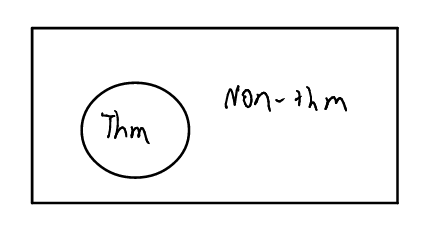
\includegraphics[width=.9\linewidth]{./Images/i5.png}
\end{center}
\begin{itemize}
\item In GEB, he calls the circle the figure and the ground the non-thms that are the non-thms of the circle but they are theorems themselves.
\item Recursive sets are decidable. Why?
\item Can a set be recursively enumerable but not recursive?
\end{itemize}
\section{Lecture 8 \textit{<2017-09-28 Thu>}}
\label{sec:orgdec2daa}
\subsection{Theorems}
\label{sec:org1972e10}
\(P\) is equivalent to \(Q\) relative to \(A_1\ldots A_n\):
\begin{itemize}
\item \(A_1 \ldots A_n, P\) prove \(Q\)
\item \(A_1 \ldots A_n, Q\) prove \(P\)
\end{itemize}
\subsubsection{E.g.}
\label{sec:orgb4add87}
Relative to Euclid's axioms:

Proclus' axiom
\begin{itemize}
\item If a line intersects 2 parallels it must intersect the other
\end{itemize}
Playfail's axiom
\begin{itemize}
\item If a line is parallel to a point, then there exists one parallel containing that point
\end{itemize}
Parallel postulate

Are equivalent.
\begin{itemize}
\item If you cannot prove \(P\) from \(A_1\ldots A_n\) then \(P\) is \uline{independent} of \(A_1 \ldots A_n\)
\end{itemize}

Parallel postulate is independent from the axioms of Euclid.
\begin{itemize}
\item One way to show:
\begin{itemize}
\item Give a model for \(A_1 \ldots A_n\) in which \(P\) is false. (If a model makes \(P\) false, then \(P\) cannot be a theorem.)
\end{itemize}
\item How to show that there are certain models for Euclid's axioms where the parallel postulate is false? Well, we have to come up with a model.
\end{itemize}

\begin{enumerate}
\item Playfail's axiom
\label{sec:org43597c2}
There exists exactly one parallel to a given line through a given point.
\begin{itemize}
\item What would it mean for this to be false?
\begin{itemize}
\item Playfair's axiom can be false in \(2\) ways:

a) More than one parallel exists

b) No parallel exists
\end{itemize}
\end{itemize}

b)
\begin{itemize}
\item Line -> great circle on a sphere
\end{itemize}
\begin{center}
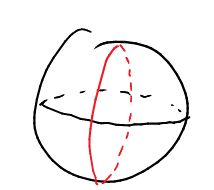
\includegraphics[width=.9\linewidth]{./Images/i6.png}
\end{center}
All great circles intersect, no parallels (Elliptic geometry)

\begin{itemize}
\item Point -> Point and it's antipode
\end{itemize}

a) 
\begin{itemize}
\item Line -> line inside disc
\item Point -> point inside the disk
\end{itemize}


Infinitely many parallel lines
(Hyperbolic geom.)

\begin{center}
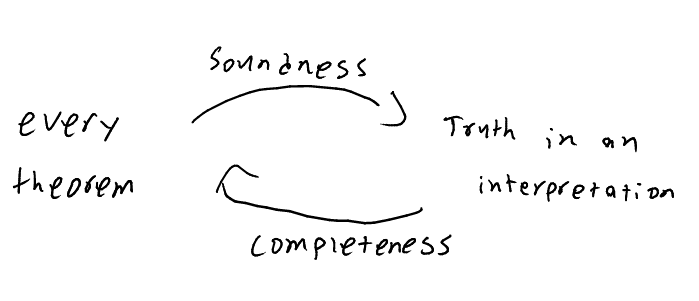
\includegraphics[width=.9\linewidth]{./Images/i8.png}
\end{center}
\end{enumerate}

\subsection{PQ*-system}
\label{sec:org10638bb}
\begin{itemize}
\item Ax. schema 1: xp\mbox{-}qx\mbox{-}
\item IR: xpyqz \(\to\) xpy-qz-
\item Ax. schema 2: xp\mbox{-}qx

\item Interpretation: 
\begin{itemize}
\item p -> plus

\item q -> equals

\item \mbox{-} -> unit
\end{itemize}

\item \mbox{-}p\mbox{-}q\mbox{-}\mbox{-}
\item Now, \mbox{-}\mbox{-}p\mbox{-}q\mbox{-}\mbox{-} is a thm
\item Meaning: 2+1 = 2, which is false.
\item Complete but not sound with respect to interpretation 1 (p -> plus)
\begin{itemize}
\item Different interpretation (2):

\begin{itemize}
\item p -> plus

\item q -> greater or equal

\item \mbox{-} -> unit

\item Sound but not complete with respect to interpretation 2.

\begin{itemize}
\item Ex. \mbox{-}\mbox{-}\mbox{-}p\mbox{-}\mbox{-}q\mbox{-} is not a theorem, but \(3+1 \geq 1\) is a truth

\item Axiom schema 2 only gives you things greater by 1
\end{itemize}
\end{itemize}

\item Different interpreation (3):

\begin{itemize}
\item p -> plus

\item q -> greater by 1 or equal

\item \mbox{-} -> unit

\item Sound and complete with respect to interpretation 3
\end{itemize}
\end{itemize}
\end{itemize}
\subsection{Propositional Logic}
\label{sec:orgfbe1365}
\begin{itemize}
\item Today's presentation is harder for those who already know propositional logic, next week will be the standard presentation.
\end{itemize}
\subsubsection{Formula trees:}
\label{sec:org4ca4b66}
\begin{itemize}
\item Language: Propositional variables: \(P_0, P_1, P_2, \ldots\)
\begin{itemize}
\item Unary connective: \(\sim\) (negation)
\item Binary connectives: \(\wedge\) (conjunction)
\begin{itemize}
\item \(\vee\) (disjunction)
\item \(\supset\) (implication)
\end{itemize}
\end{itemize}
\end{itemize}
\begin{enumerate}
\item Inductive Definition
\label{sec:org960da60}
\begin{enumerate}
\item Base clause: A prop. variable is a formula tree
\item Inductive clauses: If \(A,B\) are formula trees then \begin{center}
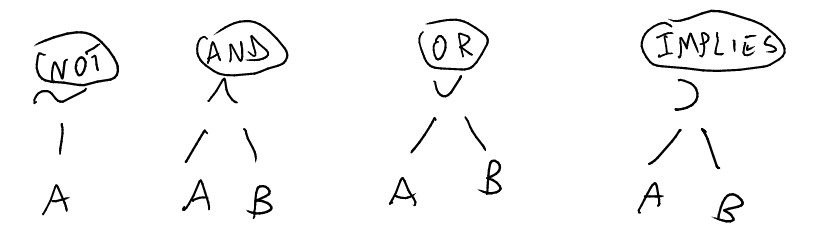
\includegraphics[width=.9\linewidth]{./Images/i9.png}
\end{center} are also formula trees (with A, B as subtrees)
\item Nothing else is a formula tree
\end{enumerate}
\item E.g.
\label{sec:orgbe0e41f}
\begin{center}
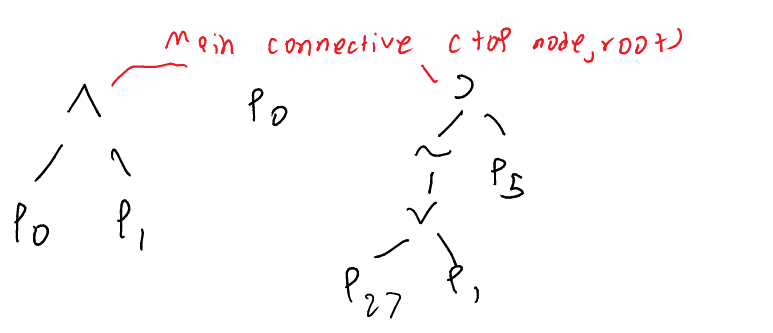
\includegraphics[width=.9\linewidth]{./Images/i10.png}
\end{center}
The tree to the right has 5 subtrees (main connective is not a subtree of itself)
\item Truth value assignment
\label{sec:orgf15973e}
A \uline{truth value assignment} is a function from propositional variables to \(\{T, F\}\) (True, False). The \uline{truth value} of a formula tree A under the truth value assignment f is:
\begin{itemize}
\item Case 1: A is a propositional variable: f(A)
\begin{itemize}
\item E.g. \(f(P_0)=T\), \(f(P_1)=F\), \(f(P_{27})=T\), \(f(P_{5})=F\)
\end{itemize}
\item Case 2: A is of the form: \begin{center}
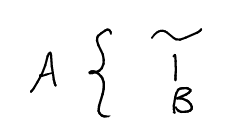
\includegraphics[width=.9\linewidth]{./Images/i11.png}
\end{center}
\begin{itemize}
\item Truth values:
\end{itemize}
\end{itemize}
\begin{center}
\begin{tabular}{ll}
B & A\\
\hline
T & F\\
F & T\\
\end{tabular}
\end{center}
\begin{itemize}
\item Case 3: A is of the form \begin{center}
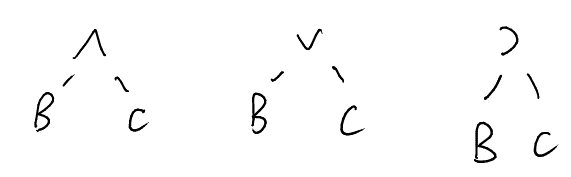
\includegraphics[width=.9\linewidth]{./Images/i12.png}
\end{center}
\end{itemize}

\begin{center}
\begin{tabular}{lllll}
B & C & A\(_{\text{1}}\) & A\(_{\text{2}}\) & A\(_{\text{3}}\)\\
\hline
T & T & T & T & T\\
T & F & F & T & F\\
F & T & F & F & T\\
F & F & F & F & T\\
\end{tabular}
\end{center}
\end{enumerate}
\section{Lecture 9 \textit{<2017-10-03 Tue>}}
\label{sec:orgc3fe77c}
\subsection{Propositional Logic}
\label{sec:org776f923}
Most of this is on handout 2b.

Let's define logic as a formal system.
\begin{itemize}
\item Alphabet: \(P_0, P_1, P_2, \ldots\) (\(\aleph_0\) propositional variables)
\item Connectives: \(\wedge\) (conjunction), \(\vee\) (disjunction), \(\supset\) (implication), \(\sim\) (negation)
\item Parentheses
\end{itemize}

\subsection{Well-formed formulas (wff)}
\label{sec:orgf438d90}
\begin{enumerate}
\item Base clause: \(P_i\) is a wff (\(i \in \mathbb{N}\)) (called atomic)
\item Inductive clause: If \(A\) and \(B\) are wffs, then so are:
\begin{itemize}
\item \(\sim A\) "not"
\item \((A \wedge B)\) "and"
\item \((A \vee B)\) "or"
\item \((A \supset B)\) "implies"
\end{itemize}
\item Nothing else is.
\end{enumerate}

E.g. 
\begin{itemize}
\item \(P_0\supset P_1\) is \textbf{not well formed}, lack of parentheses.
\item \((P_0\supset P_1)\)
\item \((P_{27})\) is \textbf{not well formed}, shouldn't have parentheses in atomic form.
\item \((\sim P_1 \wedge \sim (P_0 \supset P_2))\)
\item Can be shown as: \begin{center}
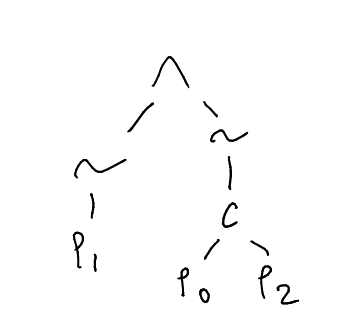
\includegraphics[width=.9\linewidth]{./Images/i13.png}
\end{center}
\end{itemize}
Convention: outer parens are omitted (except if asked for a well formed expression explicitly, as parentheses are required to comply with rules that give us the nice structure)
\subsubsection{Interpretation}
\label{sec:orgc9b661e}
Propositional variables \(\to\) truth values: 
\begin{center}
\begin{tabular}{ll}
True & False\\
\hline
T & F\\
1 & 0\\
T & \(\perp\)\\
\end{tabular}
\end{center}

(Bivalence)

\subsubsection{Truth tables}
\label{sec:org7b62472}
A,B (metavariables that stand for wff):
\begin{center}
\begin{tabular}{lllll}
A B & A \(\wedge\) B & A \(\vee\) B & \(\sim\) A & A \(\supset\) B\\
\hline
T T & T & T & F & T\\
T F & F & T & F & F\\
F T & F & T & T & T\\
F F & F & F & T & T\\
\end{tabular}
\end{center}
\begin{itemize}
\item \(A \supset B\) -> if \ldots{} then \ldots{}
\begin{itemize}
\item A is the antecedent
\item B is the consequent
\item This is material implication, not causal implication
\item The light (B) can be on even if I didn't flip the switch (A)
\end{itemize}
\item Ex.
\end{itemize}
\begin{center}
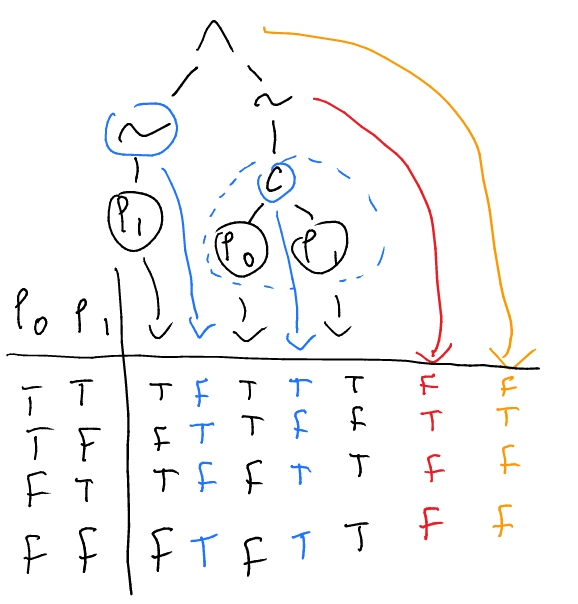
\includegraphics[width=.9\linewidth]{./Images/i14.png}
\end{center}

\begin{center}
\begin{tabular}{llll}
\(P_1\) & \(\wedge\) & \(\sim\) & \(P_1\)\\
\hline
T & F & F & T\\
F & F & T & F\\
\end{tabular}
\end{center}


\begin{center}
\begin{tabular}{llll}
\(P_1\) & \(\vee\) & \(\sim\) & \(P_1\)\\
\hline
T & T & F & T\\
F & T & T & F\\
\end{tabular}
\end{center}
Something that is always true is a \textbf{tautology}.
\begin{itemize}
\item Two wff are \uline{logically equivalent} if their TV agrees on all possible TV-assignments:
\end{itemize}
\begin{center}
\begin{tabular}{lll}
A B & A \(\supset\) B & \(\sim\) A \(\vee\) B\\
\hline
T T & T & T\\
T F & F & F\\
F T & T & T\\
F F & T & T\\
\end{tabular}
\end{center}

Do we read \(\sim A \vee B\) as \((\sim A) \vee B\) or \(\sim(A \vee B)\)?
\begin{itemize}
\item \((\sim A)\vee B\) due to the way we defined wff
\end{itemize}

Minimal sets of connectives: 
\begin{itemize}
\item \(\{\sim, \vee \}\)
\item \(\{\sim, \wedge\}\)
\item \(\{\sim, \supset\}\)
\item \(\implies\) Sheffer-Stroke
\end{itemize}

For a wff with \(n\) prop. vars, the truth table has \(2^n\) lines.

Is finding out if a proposition is a tautology decidable or not? Yes, just write out the truth table.
\subsubsection{Inferences}
\label{sec:orgd984a39}
An inference is \textbf{valid} if it is impossible for all the premises to be true and the conclusion false at the same time.

\begin{center}
\begin{tabular}{lll}
 & Premises & Conclusion\\
\hline
A B & A A \(\supset\) B & B\\
T T & T T & T\\
T F & T F & F\\
F T & F T & T\\
F F & F T & F\\
\end{tabular}
\end{center}
This is a valid inference, when both premises are true, the conclusion is also true. Thus:
\begin{itemize}
\item A, A \(\supset\) B \(\models\) B
\begin{itemize}
\item Where \(\models\) is the (semantic) consequence
\item Can check if something is semantically implied by checking the truth table and when all premises are true.
\end{itemize}
\end{itemize}
Generalizing: \(A_1, \ldots A_n \models B\)
\begin{itemize}
\item \(\models\) B (tautology)
\end{itemize}
\subsubsection{Natural Deduction (Syntax)}
\label{sec:orgc7261b8}
Introduced by Gentzen, 1934.

\(\frac{\text{Premises}}{\text{Conclusion}}\)
\begin{itemize}
\item \(\frac{A \ A \supset B}{B} \supset\) Elimination (Implication Elimination) or MODUS PONENS
\item \(\frac{A \ B}{A \wedge B} \wedge\) Introduction (since it introduces conjunction)
\item \(\frac{A\wedge B}{A}\wedge\) Elim
\item \(\frac{A \wedge B}{B}\wedge\) Elim
\begin{itemize}
\item Not the same as the rule above! You cannot get to \(B\) from the first one, you must use this one.
\item Also, \(A \wedge B\) and \(B \wedge A\) are not the same! They might have the same meaning, but they are different as strings, syntactically
\end{itemize}
\item \(\frac{A}{A \vee B}\vee\) Intro
\item \(\frac{A}{B \vee A}\vee\) Intro
\end{itemize}
Missing: 
\begin{itemize}
\item \(\vee\) Elim
\item \(\supset\) Intro
\item \(\sim\) Intro
\item \(\sim\) Elim
\end{itemize}
\section{Lecture 10 \textit{<2017-10-05 Thu>}}
\label{sec:orgfa1df29}
\subsection{Natural Deduction}
\label{sec:orgb36fada}
\begin{itemize}
\item Proof system for propositional logic
\item In the land of syntax when we do this
\begin{itemize}
\item Remember that if something looks different, it is different
\item \(A \wedge B\) is not the same as \(B \wedge A\)!
\end{itemize}
\end{itemize}

\noindent\rule{\textwidth}{0.5pt}
Some rules:
\begin{itemize}
\item \(\frac{A \ A\supset B}{B}\supset Elim\)
\item \(\frac{A \ B}{A\wedge B}\wedge Intro\)
\item \(\frac{A \wedge B}{A}\wedge ElimR\)
\item \(\frac{A \wedge B}{B}\wedge ElimL\)
\item \(\frac{A}{A \vee B}\vee Intro\)
\item \(\frac{A}{B \vee A}\vee Intro\)
\end{itemize}
Note that \(A, A \supset B \models B\) consists of semantics, not \textbf{syntax}. The above rules mentioned are rules to infer other things syntactically.

\(\frac{\frac{A \wedge B}{B}\wedge ElimL \ \frac{A \wedge B}{A}\wedge ElimR}{B \wedge A}\wedge Intro\) can be abbreviated as:
\(A \wedge B \vdash_{ND} B \wedge A\) (ND stands for natural deduction, don't confuse this symbol with the semantic one)
\begin{itemize}
\item If you can get from \(A\) to \(B\), then you can box A (canceling this assumption \(A\)) with a subscript of the amount of steps.
\end{itemize}
\begin{center}
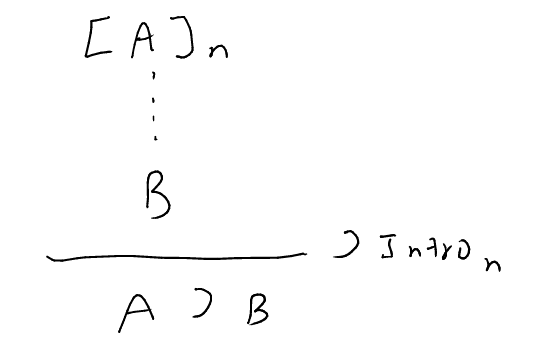
\includegraphics[width=.9\linewidth]{./Images/i15.png}
\end{center}
\begin{itemize}
\item \(\underbrace{\frac{[A]_2 \ [B]_1}{\frac{B \supset A}{A \supset (B \supset A)}\supset Intro_2} \supset Intro_1}_{\vdash_{ND} A \supset (B \supset A)}\)
\begin{itemize}
\item A and B don't prefix \(\vdash\) since they were eliminated (boxed)
\item You can get final result from no assumptions
\end{itemize}
\item \(\underbrace{\frac{A \ [B]_1}{B \supset A}\supset Intro_1}_{A \vdash_{ND} B \supset A}\)
\begin{center}
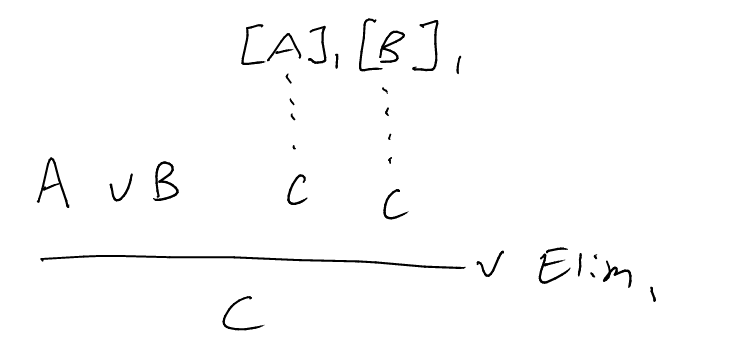
\includegraphics[width=.9\linewidth]{./Images/i16.png}
\end{center}
\item A and B both have subscript 1 because they're eliminated at the same time
\item This is like a formal definition for a proof by cases
\end{itemize}
\subsection{Exercise}
\label{sec:orgdaf5668}
Prove: \(A\vee C, A \supset B, C \supset D \vdash_{ND} B \vee D\)
\begin{center}
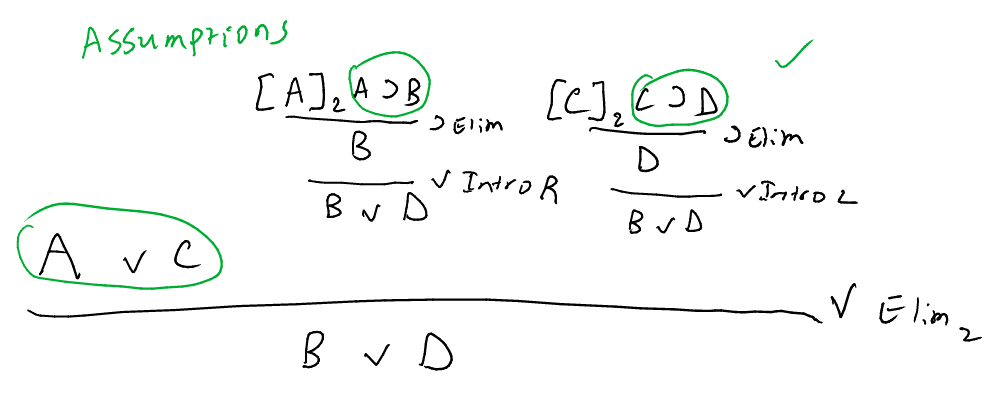
\includegraphics[width=.9\linewidth]{./Images/i17.png}
\end{center}

\noindent\rule{\textwidth}{0.5pt}
\begin{itemize}
\item New symbol: \(\perp\) false/falsum
\item Generated by:
\begin{itemize}
\item \(\frac{A \ \sim A}{\perp}\sim Elim\)
\end{itemize}
\item Can use to:
\begin{itemize}
\item \(\frac{\perp}{A}Ex falsum\) (can introduce anything)
\end{itemize}
\item \begin{center}
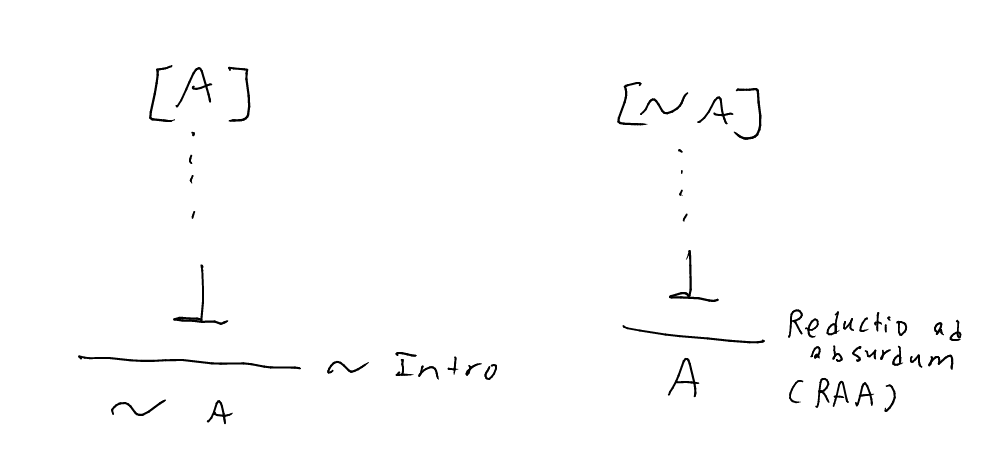
\includegraphics[width=.9\linewidth]{./Images/i18.png}
\end{center}
RAA is a proof by contradiction.
\end{itemize}
Prove: \(\vdash_{ND}\sim A \supset (A \supset B)\)
\section{Lecture 11 \textit{<2017-10-10 Tue>}}
\label{sec:org1455f40}
\subsection{Recap}
\label{sec:org41a8713}
\begin{itemize}
\item A, A \(\supset\) B \(\models\) B
\begin{itemize}
\item It is impossible for \(B\) to be false and \(A\) and \(A\supset B\) to be true.
\end{itemize}
\item A, A \(\supset\) B \(\vdash_{ND}\) B
\begin{itemize}
\item \(\frac{A \ A \supset B}{B}\supset E\)
\item How many rules in natural deduction system? About 10. How many axioms? None.
\end{itemize}
\end{itemize}
\subsection{Axiomatic Proof System}
\label{sec:orgf689c97}
\begin{itemize}
\item IR: From A and A \(\supset\) B, infer \(B\) (MODUS PONENS)
\item Substitution rule: Any wff can be substituted for A, B, C
\item Axiom schemata: (has meta variables, infinitely many axioms. Difference between axioms is important, good quiz question)
\begin{enumerate}
\item \(\sim A \supset (A \supset B)\)
\item \(B \supset (A \supset B)\)
\item \((A \supset B) \supset ((\sim A \supset B) \supset B)\)
\item \((A \supset (B \supset C)) \supset ((A \supset B) \supset (A \supset C))\)
\item \((A \supset (B \supset (A \wedge B)))\)
\item \((A \wedge B) \supset A\)
\item \((A \wedge B) \supset B\)
\item \(A \supset (A \vee B)\)
\item \(B \supset (A \vee B)\)
\item \(((A \vee B) \wedge \sim A)\supset B\)
\end{enumerate}
\item Don't need to memorize these axioms or the natural deduction rules. Will be given on an exam if required.
\item A \uline{proof} of \(A\) from assumptions \(A_1,\ldots, A_n\) is a sequence of wffs such that each element of the sequence is:
\begin{enumerate}
\item An instance of an axiom
\item An assumption (since it's a proof from assumptions)
\item The result of MP (the inference rule) to earlier elements in the sequence
\end{enumerate}
\item 1 \& 2 are base clauses, 3 is the inductive clause. This is a recursive definition. Since proofs are defined inductively, we can prove things about proofs using induction.
\end{itemize}

\uline{Prove}: A \(\supset\) A \(\vdash_{AX}\) B \(\supset\) \((A \supset A)\)
\begin{enumerate}
\item \(A \supset A\) Assumption
\item \((A \supset A)\supset (B \supset (A \supset A)) \ Ax2 [(A\supset A/B, B/A)\)]  \((A \supset A)\) replaces B in the axiom, \(B\) replaces \(A\) in the axiom.
\item \(B \supset (A \supset A)\) MP on 1 and 2
\end{enumerate}
\uline{Prove}: \(A \supset (B \supset C) \vdash_{AX} (A \supset B) \supset (A \supset C)\)
\begin{enumerate}
\item \(A \supset (B \supset C)\) Assumption
\item \((A \supset (B \supset C)) \supset ((A \supset B) \supset (A \supset C))\) Ax 4
\item \((A \supset B) \supset (A \supset C)\) MP 1,2
\end{enumerate}
\subsection{GEB proof system}
\label{sec:org72ca491}
\subsubsection{Ex.}
\label{sec:org937a133}
\(\vdash_{ND} (A \wedge B) \supset (B \wedge A)\)
\begin{itemize}
\item \(\frac{\frac{A \wedge B}{B}\wedge Elim \ \frac{A \wedge B}{A} \wedge Elim}{\frac{B \wedge A}{(A \wedge B) \supset (B\wedge A)} \supset Intro}\wedge Intro\)
\end{itemize}
\(\vdash_{GEB} (A \wedge B) \supset (B \wedge A)\)
[ push
\begin{itemize}
\item \(A \wedge B\) ass
\item \(A\) sep
\item \(B\) sep
\item \(B \wedge A\) joining
\end{itemize}
] pop
\((A \wedge B)\supset (B \wedge A)\)
\begin{itemize}
\item Won't go over GEB system in class, not as interesting, but you can look it over in handout or in GEB.
\end{itemize}
\subsection{Relations of systems}
\label{sec:org8300da2}
How do these 3 systems relate to each other?

What we have so far: 
\begin{enumerate}
\item Semantic consequence: \(\Gamma \models A\), read as \(\Gamma\) \uline{entails} \(A\) or \(A\) is a \uline{logical consequence} of \(\Gamma\)  
\begin{itemize}
\item Check via \uline{truth tables}
\end{itemize}
\item Syntactic: \(\Gamma \vdash A\), read as \(\Gamma\) \uline{proves} \(A\) or \(A\) is \uline{derivable} from \(\Gamma\)
\begin{itemize}
\item Check via natural deduction
\item or axiomatic proof
\item or GEB proof
\item All 3 are equivalent
\end{itemize}
\end{enumerate}

To show that the natural deduction system and the axiomatic system are equivalent (proofs in one system can be acquired in the other system):
\begin{enumerate}
\item Prove all axioms from the natural deduction rules. (Modus Ponens is an inference rule in natural deduction)
\item Show that each natural deduction rule corresponds to an axiomatic proof
\end{enumerate}

\noindent\rule{\textwidth}{0.5pt}
Proving axiomatic axioms:
\begin{enumerate}
\item \(\vdash \sim A \supset (A \supset B)\)
\begin{center}
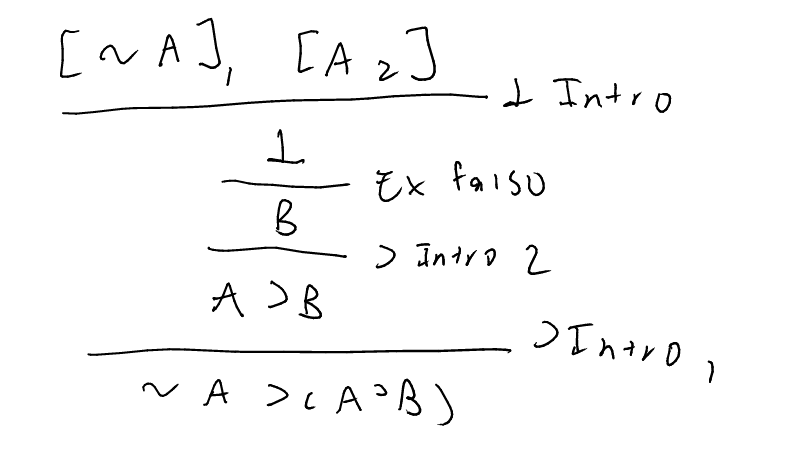
\includegraphics[width=.9\linewidth]{./Images/i19.png}
\end{center}
\item \begin{center}
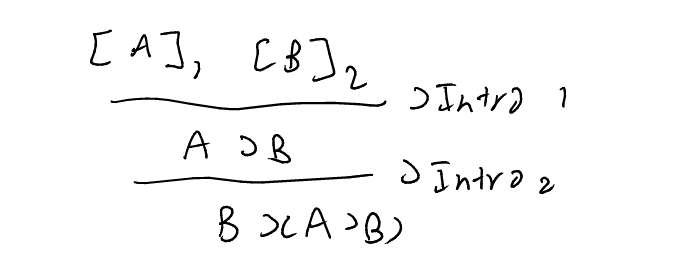
\includegraphics[width=.9\linewidth]{./Images/i20.png}
\end{center}
\end{enumerate}
You can do this for all axioms and you'll get that they're equivalent. The fact that we know they're equivalent now allows us to use which one we prefer and go from one to the other, you won't lose any logical power.

\noindent\rule{\textwidth}{0.5pt}
How does the semantic consequence relate to the syntactic consequence?
\subsubsection{Soundness Theorem}
\label{sec:org9848dc2}
If \(\Gamma\) is a set of wff and \(A\) wff then:
\begin{itemize}
\item If \(\Gamma \vdash A\), then \(\Gamma \models A\)
\item To show, show that all axioms are tautologies. We already know that modus ponens is a semantic consequence as well.
\end{itemize}
We also have if \(\vdash A\), then \(\models A\), i.e. if derivations with no or closed assumptions, then tautology, via soundness theorem.
\subsubsection{Completeness Theorem}
\label{sec:orge8755b2}
If \(\Gamma \models A\), then \(\Gamma \vdash A\)
\begin{itemize}
\item If \(A\) is a logical consequence of \(\Gamma\), then there is also a proof of \(A\) from \(\Gamma\)
\end{itemize}
Proof of these theorems done in PHIL 310 and MATH 318

if \(\models A\), then \(\vdash A\), tautologies can be derivations with no or closed assumptions
\section{Lecture 12 \textit{<2017-10-12 Thu>}}
\label{sec:orgdfc9132}
\begin{itemize}
\item There will be a proof question on the quiz (natural deduction/axiomatic)
\begin{itemize}
\item You will be given the rules, don't need to memorize
\end{itemize}
\item Most important thing is terminology
\end{itemize}
\subsection{Recap}
\label{sec:org705bf1d}
\begin{itemize}
\item Propositional logic
\begin{itemize}
\item Syntax (formula trees):
\begin{itemize}
\item Language
\item (Inference) rules
\item Proof-systems
\end{itemize}
\item Semantics:
\begin{itemize}
\item Truth tables
\end{itemize}
\item Soundness and completeness theorem (connects them)
\end{itemize}
\item Now we will be doing the same thing (structurally), but we'll be doing first order logic
\begin{itemize}
\item No truth tables, but structures and interpretations instead
\end{itemize}
\end{itemize}
\subsection{First Order Logic (FOL)}
\label{sec:org932683d}
Language \(\frak{L}\) of FOL:
\begin{enumerate}
\item Variables: \(X_0, X_1, X_2, \ldots\)
\item n-ary (can have \(n\) arguments) function symbols: \(f_0, f_1, f_2, \ldots\)
\begin{itemize}
\item 0-ary fun symbols: \uline{constant}, don't take in any arguments
\end{itemize}
\item Predicate symbols (n-ary): \(P_0, P_1, P_2\)
\item Pred. symbol \(=\)
\item Propositional connectives: \(\wedge, \vee, \supset, \sim, \perp\)
\item Quantifiers: \(\forall\) ("for all", universal), \(\exists\) ("exists", existential)
\item Parentheses: \(()\)
\end{enumerate}
2 and 3 are called extra-logical, since they aren't fixed, need to be given meaning, must be interpreted when we give the semantics.

Expressions: 
\begin{center}
\begin{tabular}{ll}
Prop. & FOL\\
\hline
wff - T/F & wff - T/F\\
 & Terms - like names\\
\end{tabular}
\end{center}

\subsubsection{Term}
\label{sec:orgfd5a2e1}
Def. A \uline{term} is 
\begin{enumerate}
\item A variable is a term
\item If \(f\) is an n-ary fun symbol, and \(t_1,\ldots,t_n\) are terms, then \(f(t_1,\ldots,t_n)\) is a term.
\item Nothing else.
\end{enumerate}

Sometimes write \(t_1 f t_2\) for \(f(t_1,t_2)\) (infix notation for binary function symbols)
\subsubsection{wff}
\label{sec:orgbecfff9}
A \uline{wf-formula}
\begin{enumerate}
\item If \(P\) is an n-ary predicate symbol, \(t_1, \ldots, t_n\) are terms, then \(P(t_1, \ldots, t_n)\) is a wff. (atomic formula)
\begin{itemize}
\item In particular: \(t_1 = t_2 = (t_1, t_2)\) is wff
\end{itemize}
\item If \(A, B\) are wff then \(\sim A, (A \vee B), (A \wedge B), (A \supset B)\) (we see that propositional logic is built into first order logic)
\item If \(A\) is a wff, x a variable, then
\begin{itemize}
\item \((\forall x : A)\) and \((\exists x : A)\) are wff. Here, \(A\) is called the scope of the quantifier.
\end{itemize}
\item Nothing else.
\end{enumerate}
\subsubsection{First Order Arithmetic (FOA)}
\label{sec:orge3ca627}
\begin{itemize}
\item Going to be using this a lot
\end{itemize}
To use FOL, you must specify the language \(\frak{L}\) which describes the function symbols.
\begin{enumerate}
\item Syntax
\label{sec:org3bcdcb9}
\begin{itemize}
\item Fun symbols:
\end{itemize}
\begin{center}
\begin{tabular}{lrlll}
\hline
Arity & 0 & 1 & 2 & 2\\
 & 0 & S & \(+\) & \(x\)\\
 & Zero symbol & Successor symbol & Plus & Times\\
 & Constant & S(x) & \(t+t\) & \(t\times t\)\\
\end{tabular}
\end{center}
\begin{itemize}
\item Terms: Ex: \(s(s(0)),x_1,0, +(x_1,x_2), 0 \times S(0)\)
\item Formulas: \(x_1 = x_2\) (Since a formula involves a predicate symbol and the only predicate symbol we have is \(=\))
\begin{itemize}
\item \(0=(x_1+x_2)\)
\item \(\sim(0 = (x_1+x_2))\)
\item \((x_1 = x_2) \supset \sim(0 = (x_1+x_2))\)
\item \((\forall x_1 : x_1 = 0)\)
\item \((\exists x_1 : x_1 = 0)\)
\item These can all be true or false depending on what we're talking about
\end{itemize}
\end{itemize}
\item Semantics
\label{sec:org4bda286}
Structure = <universe of discourse; designated elements from UD (constants); n-ary operations (fun symbols); n-ary relations (predicate symbols)>
\begin{itemize}
\item Structure depends on language you want to interpret. If your language has no constants, you won't need designated elements. If you have 5 fun symbols, you'll need 5 n-ary operations, etc.
\item An interpretation of a language \(\frak{L}\), is a structure and a mapping \(\sigma\) of the extra-logical symbols into the structure.
\item An interpretation of FOA: 
\begin{itemize}
\item \(\frak{n}=\) <natural numbers; zero; successor; addition; multiplication> (natural number structure, how it was made to be interpreted. But you can interpret it differently. You can swap the mapping, but make sure they have the same arity: can switch addition with multiplication, but not successor with zero)
\item \(\frak{L}\): 0 s \(+\) \(\times\)
\item Map: 0 -> \(0\), s -> successor, \(+\) -> addition\((+)\), \(\times\) -> multiplication \((\times)\)
\begin{itemize}
\item Make sure to understand the difference between the semantic level and the syntactic level. They look the same, one is the symbol and one is the meaning. One is the symbol for addition, but the other means addition.
\item Why don't we have n-ary relations? Because FOA has no predicate symbols. Shows how structure is dependent on language.
\item \(\times^{\sigma}=\sigma(\times)=\) mult, shows what \(\times\) maps to in mapping \(\sigma\)
\end{itemize}
\end{itemize}
\end{itemize}
\item Truth in a structure (Tarski 1933)
\label{sec:org119df11}

(T1) If x is a variable, then \(x^{\sigma}\) is given by the \uline{valuation} (interpretation that also interprets the variables, i.e. map \(x_1\), \(x_2\), etc.).

(T2) If f is an n-ary function symbol, \(t_1,\ldots,t_n\) terms:
\begin{itemize}
\item \((f(t_1,\ldots, t_n))^{\sigma} = f^{\sigma}(t_1^{\sigma},\ldots ,t_n^{\sigma})\)
\begin{itemize}
\item e.g. \([s(s(0))]^{\sigma} = s^{\sigma}([s(0)]^{\sigma}) = s^{\sigma}(s^{\sigma}(0^{\sigma}))\)
\end{itemize}
\end{itemize}
(F1) \(P\) nary predicate symbol, \(t_1, \ldots , t_n\) terms
\begin{equation*}
(P(t_1, \ldots, t_n))^{\sigma} = 
\begin{cases}
T & \text{if $P^{\sigma}$ holds of $t_n^{\sigma}, \ldots, t_n^{\sigma}$} 
\\ F & \text{otherwise}
\end{cases}
\end{equation*}
(F2) 
\begin{equation*}
(\sim A)^{\sigma} =
\begin{cases} 
T & \text{ if $A^{\sigma}$}=F
\\ F & \text{ otherwise}
\end{cases}
\end{equation*}
(F3) 
\begin{equation*}
(A\supset B)^{\sigma} = 
\begin{cases}
T & \text{ if $A^{\sigma}=F$ or $B^\sigma = T$}
\\ F & \text{ if $A^{\sigma}=T$ and $B^{\sigma}=F$}
\end{cases}
\end{equation*}
(F4) 
\begin{equation*}
(\forall x : A)^{\sigma} = 
\begin{cases}
T & A^{\sigma(u/x)}=T \text{ for all }u \in UD
\\ F & \text{otherwise}
\end{cases}
\end{equation*}
\end{enumerate}
\section{Lecture 13 \textit{<2017-10-17 Tue>}}
\label{sec:org049c3cf}
\subsection{Quiz Review}
\label{sec:orgb226f3f}
\begin{itemize}
\item Inductive definition of Strings
\item Prime numbers recursive? Yes
\item Tautology, semantic
\item Proof system, syntactic
\item Derivation, syntactic
\item Truth table, semantic
\item Inference rule, syntactic
\item How do you know something can be proved by something? Use Completeness theorem and check truth table
\end{itemize}
\subsection{Tarski \& Quantifiers}
\label{sec:org30bbad8}
\begin{equation*}
  (\forall x: A)^{\sigma} =
  \begin{cases}
    T & A^{\sigma(u/x)}=T \text{ for every }
    u \in UD
    \\ F & \text{otherwise}
  \end{cases}
\end{equation*}
\begin{equation*}
  (\forall x:\sim (0=Sx))^{\sigma (u/x)} = T \text{ for every }u \in \mathbb{N}
\end{equation*}
How to check this?

Decompose
\begin{align*}
  (\sim (0=Sx))^{\sigma (u/x)} = T \text{ for every }u \in \mathbb{N}
  \\ (0=Sx)^{\sigma (u/x)} = F \text{ for every }u \in \mathbb{N}
  \\ (\textbf{0 = succ u}) = F \text{ for every }u \in \mathbb{N}
\end{align*}
False for every \(u \in \mathbb{N}\), \(succ 0 \neq 0, succ 1 \neq 0, \ldots\)

Can then define the following:
$$\exists x : A \iff \sim \forall x : \sim A$$
Read as "there exist an x \ldots{}"

If one wanted to define it formally like the universal quantifier:
\begin{equation*}
  (\exists x : A)^{\sigma} =
  \begin{cases}
    T & \text{if } A^{\sigma(u/x)}=T \text{ for at least one }u \in UD
    \\ F & \text{otherwise}
  \end{cases}
\end{equation*}

$$\forall x : \exists y : M(x,y)$$
Structure for interpretation: < all people ; is mother of>
\begin{itemize}
\item For all \(x\), there is a y, such that x is the mother of y.
\begin{itemize}
\item This is false, not everyone is a mother.
\item How can we make it true?
\end{itemize}
\end{itemize}
$$ \forall x : \exists y : M(y,x)$$
\begin{itemize}
\item Everybody has a mother, true
\end{itemize}
What does the following mean?
$$\exists x : \forall y : M(x,y)$$
\begin{itemize}
\item There exists somebody who is the mother of everybody
\begin{itemize}
\item False
\end{itemize}
\end{itemize}
$$\exists x : \forall y : M(y,x)$$
\begin{itemize}
\item There exists someone such that everyone is their mother
\end{itemize}
We see that just switching around quantifiers changes meaning completely. So we must read quantifiers correctly, from left to right.
\begin{itemize}
\item We can say:
\begin{itemize}
\item \(\overbrace{\sigma}^{\text{valuation}}\) \uline{satisfies} \(\overbrace{A}^{\text{wff}}\) : \(A^{\sigma}=T\)
\item \(\overbrace{\sigma}^{\text{valuation}}\) \uline{satisfies} \(\overbrace{\Gamma}^{\text{set of wff}}\) : \(A^{\sigma}=T\) for all \(A \in \Gamma\)
\end{itemize}
\item A is \uline{logically true}: A is satisfied by every valuation
\begin{itemize}
\item \(\models A\)
\end{itemize}
\item A is a \uline{logical consequence} of \(\Gamma\): every valuation that satisfies \(\Gamma\) also satisfies \(A\)
\begin{itemize}
\item \(\Gamma \models A\)
\end{itemize}
\item \(\Gamma\) unsatisfiable, no valuation that satisfies each \(A \in \Gamma\) at the same time
\item These are similar to what was said in propositional logic, but with different terms
\end{itemize}
This was all in the land of semantics (we talked about truth). Now we'll go back to the land of syntax.
\subsection{Syntax}
\label{sec:orgf2dc034}
Variable \(x\) is bound if it falls in the scope of a quantifier that has \(x\) as a variable of quantification. \(x\) is quantified in \(A\).
$$\forall x : \overbrace{\underbrace{A}_{\text{scope}}}^{\text{$x$ is bound in $A$}}$$
$$ \forall x_1 : \exists x_2 : (x_1 = x_2 + x_3)$$
\begin{itemize}
\item \(x_1\) and \(x_2\) are bound variables, while \(x_3\) is a free variable.
\end{itemize}
$$ (\forall x_1 : \exists x_2 : (x_1 = x_2 + x_3)) \vee (\underbrace{x_1}_{\text{free}} = 0)$$
The second \(x_1\) is free since it's not in the scope of the quantifier.
$$ \forall x_1 : \exists x_2 : (x_1 = x_2 + x_3) \vee (\underbrace{x_1}_{\text{free}} = 0)$$
In this case, both \(x_1\) are bound.
\section{Lecture 14 \textit{<2017-10-19 Thu>}}
\label{sec:org7734fc4}
\begin{itemize}
\item Good midterm question: What does \(\Gamma \models A\) mean in one sentence?
\begin{itemize}
\item \(\Gamma\) is a set of wff and \(A\) is a wff. \(\Gamma \models A\) if everything in \(\Gamma\) is true then \(A\) is true or it is impossible that everything in \(\Gamma\) is true and \(A\) isn't
\end{itemize}
\item \(\Gamma \vdash A\)
\begin{itemize}
\item There's a proof of \(A\) from \(\Gamma\)
\end{itemize}
\item \(\Gamma \models A\) (What does this mean in FOL?)
\begin{itemize}
\item \(\Gamma\) entails \(A\)
\item Every valuation that satisfies \(\Gamma\) satisfies \(A\)
\begin{itemize}
\item A lot harder to check than propositional logic, since you have to check \textbf{every} valuation
\end{itemize}
\end{itemize}
\end{itemize}
\subsection{FOA}
\label{sec:org0e2ceb0}
If UD \(= \mathbb{N}\), Even(x) \(\implies\) even
\begin{itemize}
\item What does: \(\exists x \ Even(x)\) mean?
\begin{itemize}
\item There exists at least one number that is even.
\end{itemize}
\item \(\exists x \exists y \ Even(x) \wedge Even(y)\)
\begin{itemize}
\item There exist a \(x\) and \(y\) such that \(x\) is even and \(y\) is even
\item There exists at least an even number (\(x\) and \(y\) can be the same)
\end{itemize}
\item \(\exists x \exists y \ (Even(x) \wedge Even(y)) \wedge \sim (x = y)\)
\begin{itemize}
\item There exists at least two even numbers
\end{itemize}
\item \(\exists x \exists y \ (Even(x) \wedge Even(y)) \supset \sim (x = y)\)
\begin{itemize}
\item True, since it's exists and we can pick our \(x\) and \(y\)
\end{itemize}
\item \(\forall x: \forall y: x = y\)
\begin{itemize}
\item For all \(x\) and for all \(y\), \(x=y\)
\item False.
\item We can make this true if we use a universe of discourse with one element, such as \(UD = \{A\}\)
\end{itemize}
\item \(\forall x: \forall y: \sim (x = y) \supset [Even(x) \vee Even(y)]\)
\begin{itemize}
\item For 2 numbers that aren't equal, one of them is even
\item False
\end{itemize}
\item \(\forall x: \forall y: \sim (x = y) \supset [Even(x) \vee Even(y)]\)
\begin{itemize}
\item If two numbers aren't equal, then one is greater than the other
\item True
\end{itemize}
\end{itemize}
\subsection{Substitution}
\label{sec:org0a30bed}
Recall, a term is either a variable or a function symbol followed by the appropriate number of terms. 
\begin{itemize}
\item A term is \uline{closed} if it contains no variables.
\begin{itemize}
\item Ex. \(0, S0\) in FOA
\end{itemize}
\item Otherwise it's called open
\item \uline{Sentence}: wff with no free variables, \(0=0\), \(\forall x_1:\exists x_2: x_1=x_2\)
\item A term \uline{\(t\)} is free for an occurrence of \uline{\(x\)} in \uline{\(A\)} iff
\begin{itemize}
\item \(x\) is a free variable in \(A\)
\item And \(x\) does not lie within the scope of any quantifier, where \(y\) is a variable that appears in \(t\)
\end{itemize}
\item What do we want to do? Replace variables by terms.
\end{itemize}
\uline{Substitution}:
\begin{itemize}
\item \(s,t\) terms, \(x\) var
\item \(x(t/x) = t\)
\begin{itemize}
\item Term \(t\) replaces variable \(x\)
\end{itemize}
\item \(y(t/x) = y\)
\item \(f(s_1,\ldots,s_n)(t/x) = f(s_1(t/x),\ldots,s_n(t/x))\)
\begin{itemize}
\item Since the \(s_i\) are terms, we have to do the substitution on each term
\end{itemize}
\item \(\forall x: P(x) (t/x)\)
\begin{itemize}
\item We cannot do this, \(x\) is not a free variable
\item It isn't \(\forall t : P(t)\), because you cannot use a quantifier on a term, a term can be a constant.
\end{itemize}
\item \(\forall y : \underbrace{x}_{\text{free}}=y (y/x) \rightarrow \forall y: \underbrace{y}_{\text{bound}}=y\)
\begin{itemize}
\item These are not equivalent
\item Might end up making a false statement true, want to avoid this.
\item Don't want to switch from free to bound.
\end{itemize}
\end{itemize}
\subsection{Proofs}
\label{sec:org6d19da0}
Now we need a proof system for First Order Logic. Will see natural deduction in class, read about axiomatic and GEB on the handout.
\subsubsection{Natural deduction calculus}
\label{sec:org616d4f8}
We need introduction and elimination rules for quantifiers. 
\begin{prooftree}
\AxiomC{A(a/x)}
\LeftLabel{$\forall \ Intro:$}
\UnaryInfC{$\forall x: A$}
\end{prooftree}
Here, \(a\) is a variable/Eigen variable.
\begin{itemize}
\item e.g.
\end{itemize}
\begin{prooftree}
\AxiomC{0=a}
\UnaryInfC{$\forall x : (0 = x)$}
\end{prooftree}
\(a\) must be free for \(x\) in \(A\), cannot bind it.
\begin{prooftree}
\AxiomC{$\forall x : A$}
\LeftLabel{$\forall \ Elim$}
\UnaryInfC{A(t/x)}
\end{prooftree}
\(t\) must be free for \(x\) in \(A\)
\begin{itemize}
\item e.g.
\end{itemize}
\begin{prooftree}
\AxiomC{$\forall x:(x=x)$}
\UnaryInfC{$s0 = s0$}
\end{prooftree}
\begin{prooftree}
\AxiomC{A(t/k)}
\LeftLabel{$\exists \ Intro$}
\UnaryInfC{$\exists x: A$}
\end{prooftree}
\begin{itemize}
\item E.g.
\end{itemize}
\begin{prooftree}
\AxiomC{$\overbrace{\sim (0=S0)}^{A(0/x)}$}
\RightLabel{$t=0$, $A(x) \sim (x=S0)$}
\UnaryInfC{$\exists x : \underbrace{\sim (x = S0)}_{=A}$}
\end{prooftree}
\(A(0/x) \implies \sim (O = S0)\)

\begin{prooftree}
\AxiomC{$\exists x: A$}
\AxiomC{[A(a/x)]}
\UnaryInfC{.}
\UnaryInfC{.}
\UnaryInfC{.}
\UnaryInfC{C}
\LeftLabel{$\exists \ Elim$}
\BinaryInfC{C}
\end{prooftree}

\begin{prooftree}
\AxiomC{$\forall x: A(x)$}
\RightLabel{$\forall \ Elim$}
\UnaryInfC{$A(t)$}
\RightLabel{$\exists \ Intro$}
\UnaryInfC{$\exists x : A(x)$}
\end{prooftree}
For all \(x\), \(A(x)\) means that there exists \(x\) such that \(A(x)\)

\begin{enumerate}
\item Ex
\label{sec:org76cca12}
\(\vdash \forall x: (A(x)\supset B)\supset (\exists x: A(x)\supset B)\)
\begin{prooftree}
\AxiomC{$[\exists x: A(x)]_1$}
\AxiomC{$\forall x : A(x) \supset B$}
\RightLabel{$\forall \ Elim$}
\UnaryInfC{$A(t)\supset B$}
\AxiomC{$A(t)$}
\RightLabel{$\supset \ Elim$}
\BinaryInfC{$B$}
\RightLabel{$\exists \ Elim$}
\BinaryInfC{$B$}
\RightLabel{$\supset \ Intro_1$}
\UnaryInfC{$\exists x : A(x) \supset B$}
\RightLabel{$\supset \ Intro_2$}
\UnaryInfC{$\forall x : (A(x) \supset B)\supset (\exists x: A(x)\supset B)$}
\end{prooftree}
Complicated proof, won't have something like this on midterm (since just introduced these rules), but maybe final.
\item FOL: Sound \& Complete
\label{sec:org8907768}
Proved by Godel in 1930
\end{enumerate}
\section{Lecture 15 \textit{<2017-10-24 Tue>}}
\label{sec:orgdd3f452}
Reviewed quiz 2. 
\begin{itemize}
\item Recursive Definition
\begin{enumerate}
\item Base clause
\item Inductive clause
\item Final clause
\end{enumerate}
\item Recursive
\end{itemize}
Means that both the set and its complement are recursively enumerable (we can derive them as theorems in a proof system)
\begin{itemize}
\item Terms
\end{itemize}
Either a variable or an n-ary function with \(n\) terms
\begin{itemize}
\item Atomic wff
\end{itemize}
Formula made up of only terms and predicates
\begin{itemize}
\item Decision procedure to see if \(\Gamma \models A\)
\begin{itemize}
\item Make a truth table, see if when all of \(\Gamma\) is true, then \(A\) must be true
\end{itemize}
\end{itemize}
\section{Lecture 16 \textit{<2017-10-31 Tue>}}
\label{sec:org4d7317b}
\subsection{Typographic Number Theory (TNT)/Dedekind Peano Arithmetic (DPA)/FOA}
\label{sec:orgc379900}
Why were people so concerned with the consistency of this?

Say we start with geometry
\begin{itemize}
\item -> \(\mathbb{R}\times \mathbb{R}\) (cartesian)
\begin{itemize}
\item But then how do we know that real numbers are consistent?
\item -> \(\mathbb{Q}+(sets)\)
\begin{itemize}
\item But then what about the rational numbers?
\item -> \(\mathbb{N}\)
\begin{itemize}
\item How do we show the consistency of natural numbers and therefore the consistency of mathematics?
\item -> Logic (FREGE, invented predicate logic on the way)
\item -> Set theory (Cantor)
\end{itemize}
\end{itemize}
\end{itemize}
\end{itemize}
Hilbert's program (1920s):
\begin{itemize}
\item Blob with everything mathematicians do
\begin{itemize}
\item Arithmetic -> Formalize: FOA
\item Analysis ->
\item Set Theory -> Formalize: ZFC
\end{itemize}
\end{itemize}
Used finitary arithmetic to show consistency of all 3
\begin{itemize}
\item Can look at finite elements to prove something about the other domains that are infinite
\item Difference between DPA and FOA?
\begin{itemize}
\item There's no difference! Just different names.
\end{itemize}
\end{itemize}

\noindent\rule{\textwidth}{0.5pt}
TNT: 
\begin{itemize}
\item Language: 0, S, +, \(\times\)
\item Axioms:
\begin{enumerate}
\item \(\forall x:\sim(Sx=0)\), For all numbers successor of \(x\) is not \(0\)
\item \(\forall x: \forall y: (Sx=Sy)\supset x=y\), succ is injective
\item \(\forall x: (x+0) = x\)
\item \(\forall x : \forall y : (x+Sy) = S(x+y)\)
\item \(\forall x: (x\cdot 0) = 0\)
\item \(\forall x:\forall y:(x\cdot Sy) = ((x \cot y) +x)\)
\end{enumerate}
\end{itemize}
\subsubsection{Theorems}
\label{sec:orgbee3c5e}
A \uline{theory} \(T\) is said to be wff, s.t. \(s \in T\) iff \(T \vdash S\) (closed under deduction)
\begin{itemize}
\item A theory \(T\) is \uline{axiomatic} if there exists a recursive set \(A_k\) st
\item \(T=\{S|A \vdash S\}\)
\item A theorem is \uline{consistent} if it does not contain both \(A\) and \(\sim A\) for some wff \(A\).
\end{itemize}
\begin{center}
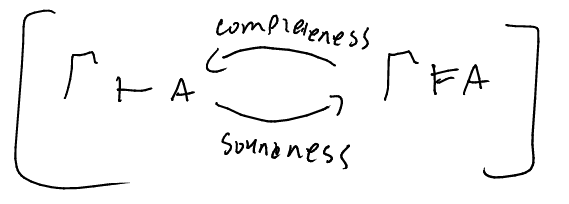
\includegraphics[width=.9\linewidth]{./Images/i21.png}
\end{center}
A theory \(T\) is \uline{complete}, if for every wff \(A\), either \(A \in T\) or \(\sim A \in T\). Both can be true, but then it'll be complete and inconsistent.

Can we come up with something not derivable from a theory?
\begin{itemize}
\item (Axioms 1.-6.) \(\nvdash \forall x: \sim(Sx = x)\)
\begin{itemize}
\item True in standard interpretation
\item Claim: Cannot derive from these axioms
\item How do we show this?
\item How do we show \(\Gamma \nvDash A\)?
\begin{itemize}
\item We're looking for an interpretation. Want one that satisfies \(\Gamma\) but does not satisfy \(A\).
\item Recall that \(\Gamma \nvDash A\) means that every interpretation that satisfies \(\Gamma\) must satisfy \(A\) (no truth tables as we're no longer in propositional logic)
\item So \(\Gamma \nvDash A \implies \Gamma \nvdash A\) from soundness (opposite direction because of negation)
\end{itemize}
\end{itemize}
\item UD: \(\mathbb{N}\cup \{*\}\)
\begin{itemize}
\item 0 -> zero
\item + -> \(+^*\)
\begin{itemize}
\item \(n \in \mathbb{N}\)

\begin{tabular}{l|l l}
  $+^*$ & $n$ & $*$
  \\ \hline $n$ & $n+n$ & $*$
  \\ $*$ & $*$ & $*$
\end{tabular}
\end{itemize}

\item \(\times\) -> \(\times^*\)
\begin{itemize}
\item \(n \in \mathbb{N}\)
\end{itemize}
\begin{tabular}{l|l l l}
    $+^*$ & $0$ & $n$ & $*$
    \\ \hline $0$ & $0$ & $0$ & $*$
    \\ $n$ & $0$ & $n \times n$ & $*$
    \\ $*$ & $0$ & $*$ & $*$
\end{tabular}
\item s -> \(s^*\)
\begin{itemize}
\item \(s^*(n) = s(n)\) if \(n\in \mathbb{N}\)
\item \(s^*(*) = *\)
\end{itemize}
\end{itemize}
\end{itemize}
$$\frak{n}=\langle\mathbb{N};0,succ,+,\times\rangle$$
$$\frak{n'}=\langle\mathbb{N}\cup\{*\};0,s^*,+^*,\times^*\rangle$$
Looking at the axioms: 
\begin{itemize}
\item Is 2 true in both? Yes.
\item Checking them all you will see that all the axioms are true in \(\frak{n'}\) as well.
\item But (1.-6.) \(\nvdash \forall x: \sim (sx = x)\) is not true in the new interpretation (because \(s^*(*)=*\)), when it is true in the old one. Which is why these axioms are insufficient to prove things as simple as this.
\end{itemize}
So these are in fact not all the axioms of TNT.

\subsubsection{\(\omega-incomplete\)}
\label{sec:orgae1283f}
\begin{itemize}
\item (1.-6.) \(\nvdash (0+0=0)\)
\begin{itemize}
\item \(\ldots (0+s0=s0)\)
\item \(\ldots (0+ss0=ss0)\)
\end{itemize}
\item But \(\nvdash \forall x: (0+x=x)\) (not the same as axiom 3)
\end{itemize}
This is called \(\omega-incomplete\)

Need an additional axiom

7.Axiom schema of induction
$$A(0) \supset [\forall x:(A(x)\supset A(sx))\supset \forall x:A(x)]$$
Called a schema because it can make countably infinite amount of axioms

Now with all 6 axioms and the axiom schema we have TNT.
\section{Lecture 17 \textit{<2017-11-02 Thu>}}
\label{sec:org8d1ceff}
\subsection{MIU}
\label{sec:orge6a8289}
Is MU a MIU theorem? Recall:

I. xI -> xIU

II. Mx -> Mxx

III. III -> U

IV. UU -> \(\emptyset\)

Axiom: MI
\begin{itemize}
\item If it is a theorem, then you can prove it.
\item If it isn't though, you can do MIU proofs for the rest of your life and never know the answer
\item One way to answer this is find properties of these theorems
\end{itemize}
\subsubsection{Theorem}
\label{sec:org797a684}
The number of I's in a MIU theorem is not a multiple of \(3\) (and \(0\) is a multiple of \(3\), so if this follows then MU is not a theorem)
\subsubsection{Proof by strong induction}
\label{sec:org13e3a69}
\begin{itemize}
\item Let \(t\) be a theorem, obtained from a proof of length \(n\) (theorem at line \(n\) of our proof)
\item IH. The I-count of all theorems in lines \(1-(n-1)\) is not a multiple of \(3\)
\item Show: Claim holds for line n
\end{itemize}
t can be:
\begin{enumerate}
\item An axiom: MI: \(1\) is not a multiple of \(3\)
\item \(t\) is obtained by Rule I from theorem \(s\) (\(1\leq s < n\)). By IH. the I-count of \(s\) is not a multiple of \(3\). So the I-count of \(t\) is also not a multiple of \(3\).
\item \(t\) is obtained by Rule II \ldots{}
\item \(t\) is obtained by Rule III \ldots{}
\item \(t\) is obtained by Rule IV \ldots{}
\end{enumerate}
Conclusion: The claim holds.

So we get the answer, to is MU a MIU-theorem -> No, because \(0\) is a multiple of \(3\). This here is a proof about proofs, which we'll be seeing a bit more of later with proofs about proofs in the TNT system.

\subsection{G$\backslash$"odel numbering}
\label{sec:org47d7fe6}
Continuing with the MIU system:
\begin{itemize}
\item We have the symbols
\begin{itemize}
\item M->3
\item I->1
\item U->0
\end{itemize}
\end{itemize}
Now we can use these proofs for arbitrary strings
\begin{center}
\begin{tabular}{rlll}
1. & MI & Axiom & \(31\) (Godel \#)\\
2. & MII & Rule II & \(311\)\\
3: & MUI & Rule II & \(3111\)\\
4. & MUI & Rule III & \(301\)\\
5. & MUIU & Rule I & \(3010\)\\
\end{tabular}
\end{center}
\(5\) can be represented as -> a) x1 -> x10 (typographical) ; b) A number whose remainder, when divided by 10 is 1, can be multiplied by 10.
\begin{itemize}
\item Two ways of talking about it once we transform it into a number.
\end{itemize}

So G$\backslash$"odel Numbering allows us to go from a formal system to number theory. 
\begin{center}
\begin{tabular}{ll}
Formal System -> & Number Theory\\
\hline
MIU & \\
MIU-thm & MIU-producible numbers\\
\end{tabular}
\end{center}
MIU-producible numbers are recursively enumerable, since we can get them from the MIU formal system   

But a more interesting transition is going from Number theory to FOA/TNT, another formal system.
\begin{center}
\begin{tabular}{ll}
Number Theory -> & FOA/TNT (formal system)\\
\hline
e.g. 2 -> & SSO\\
MIU-producible numbers & theorems\\
\end{tabular}
\end{center}

\begin{center}
\begin{tabular}{lll}
FS & Number Theory & FOA\\
\hline
MU is a MIU-thm & \(30\) is a MIU-prod. number & \(MON(\overbrace{SS \ldots S}^{30}0)\) is a TNT-theorem\\
\end{tabular}
\end{center}
MON is a predicate standing for the MIU-producible numbers. Looks something like \(\forall x : \exists y : \ldots\).
Can look specifically at one system to show it for another. Like a translation, but nothing is lost.

Now let's start with the TNT system:
\begin{center}
\begin{tabular}{lll}
Formal System & Number Theory & FOA\\
\hline
TNT &  & \\
TNT-thm & TNT-producible numbers & theorems\\
\_ is a TNT-thm & \_ is a TNT-prod.number & \_\\
\end{tabular}
\end{center}

How do we talk about the English language? "short" is short.

\begin{itemize}
\item TNT-formula: \(\forall a : \sim Sa = 0\) is a theorem of TNT
\item Go \#: 626 262 636 223 123 262 111 666 is a TNT number -> \(F(SS\ldots S0)\) is a TNT-thm
\item -> \(\sim F(G)\) is a TNT-thm -> says that "I am not a TNT-thm"
\end{itemize}
Can go from TNT to number theory to TNT. Reaching something different in the end will lead us to G$\backslash$"odel's theorem

In a TNT proof, every line can be mapped to a Godel \# (since you can translate formulas into numbers) and then you can get a unique Godel number for an entire proof

TNT-PROOF-PAIR(x,y): Predicate between a pair of numbers. True if x codes (is the godel number of) a proof of the wff coded by y

TNT-PROOF(x): \(\exists y:TNT-PROOF-PAIR(y,x)\)
\section{Lecture 18 \textit{<2017-11-07 Tue>}}
\label{sec:orge562197}
\subsection{Turing Machines}
\label{sec:org5b9565b}
\begin{itemize}
\item Formalizations of computability
\begin{itemize}
\item What is computable? Need some sort of handle on studying this mention, formalizing is a good way to do so, you can then check if something is valid in the formal system or not valid. Can also meta-reason about them and such.
\end{itemize}
\item Different formal systems for computability have been made
\begin{enumerate}
\item Representability in FOA
\begin{itemize}
\item If it can be represented in FOA it's computable
\end{itemize}
\item Arithmetic descriptions: \(\mu-\text{recursive fun}\)
\item \(\lambda-\text{calculus}\)
\item Machine-like descriptions: TM, Post, register
\end{enumerate}
\end{itemize}
These 4 were done in 1930s. All 4 can be proved to be equivalent.
\begin{itemize}
\item Going from these formal systems to computability (and vice versa) is sometimes called the Church-Turing thesis
\begin{itemize}
\item Can this be proved? No, because the Church-Turing thesis isn't well posed, going from something formal to something informal (computability). How can you go from one to the other? That's why it's a thesis not a proof.
\end{itemize}
\item Alan Turing (1912-1954) invented Turing Machines in 1936
\end{itemize}

\noindent\rule{\textwidth}{0.5pt}
Say you have a paper with numbers on it:
\begin{center}
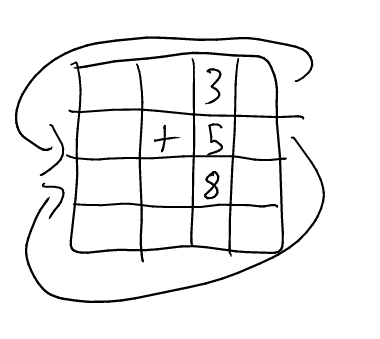
\includegraphics[width=.9\linewidth]{./Images/i22.png}
\end{center}
Conditions: 
\begin{itemize}
\item Boundedness: finite \# of symbols and possible actions
\item Locality: finite range for reading and writing
\item Tape: \begin{center}
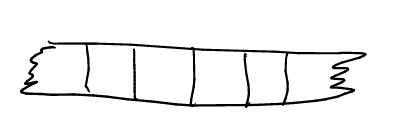
\includegraphics[width=.9\linewidth]{./Images/i23.png}
\end{center}
\begin{itemize}
\item finite alphabet, e.g. every square is either \(1\) or \(B\)(lank)
\item Head: over one square
\begin{itemize}
\item read symbol (that it's currently looking at)
\item write \& delete symbol
\item move left or right: L R
\item States: \(q_0, q_1, q_2,\ldots\)
\item Instructions:
\begin{itemize}
\item \((q_i,S_y,O_p,q_j)\)
\item \(q_i\) is current state
\item \(S_y\) is symbol read
\item \(O_p\) is operation, either \(1,B,L,R\)
\item \(q_j\) is next state
\end{itemize}
\item Always begin in state \(q_0\)
\end{itemize}
\end{itemize}
\end{itemize}
Now we can write Turing Machine programs.

TM1 = 
\begin{itemize}
\item \((q_0,B,R,q_0)\), if at a blank, go right
\item \((q_0,1,B,q_0)\), if at a 1, write a blank
\item Erases tape and never halts \begin{center}
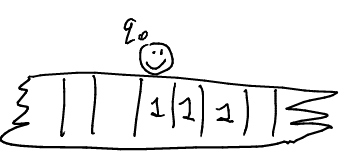
\includegraphics[width=.9\linewidth]{./Images/i24.png}
\end{center}
\item Now we want a TM that erases all 1s
\end{itemize}
TM2 = 
\begin{itemize}
\item \((q_0,1,R,q_1)\)
\item \((q_1,B,R,q_0)\)
\item Erases consecutive 1s
\item \begin{center}
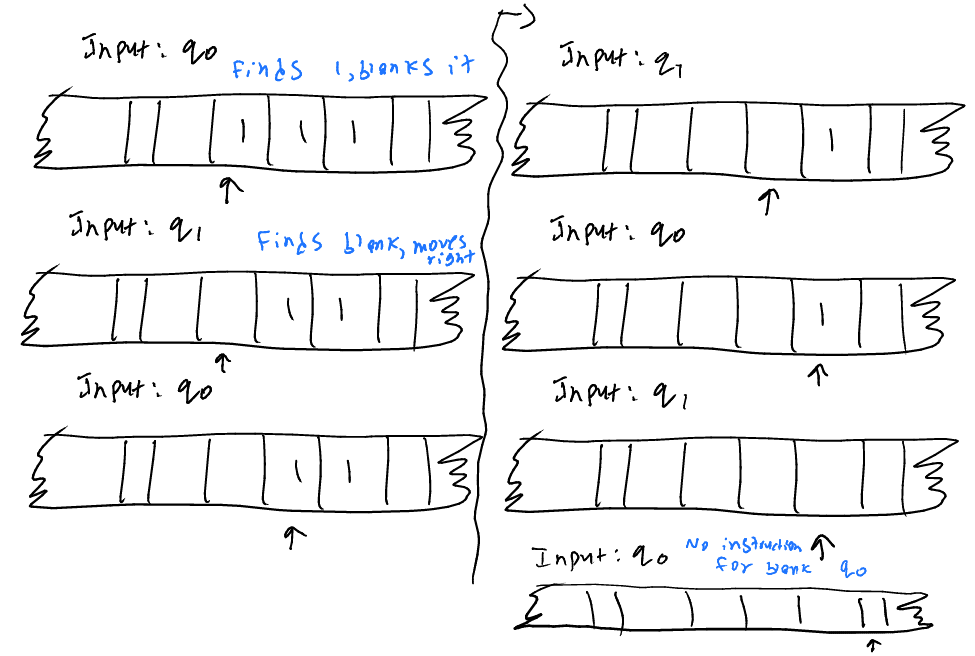
\includegraphics[width=.9\linewidth]{./Images/i25.png}
\end{center}
\end{itemize}
\subsubsection{TM as functions}
\label{sec:org835c069}
TM as functions from \(\mathbb{N}\to \mathbb{N}\) (input is only \(1\) block of consecutive \(1\)'s)
\begin{itemize}
\item \begin{center}
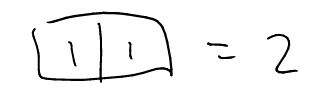
\includegraphics[width=.9\linewidth]{./Images/i26.png}
\end{center}
\item TM2: \(f(x)=0\)
\item TM3: What if we want \(f(x)=2\)
\begin{itemize}
\item Can reuse TM2, erase everything
\item Once everything is erased, write 2 \(1\)'s
\item TM3 =
\begin{itemize}
\item \((q_0,1,R,q_1)\)
\item \((q_1,B,R,q_0)\)
\item \((q_0,B,1,q_2)\)
\item \((q_2,1,R,q_3)\)
\item \((q_3,B,1,q_4)\), \(q_4\) doesn't exist, will stop at this point
\end{itemize}
\item Alternate notation:
\begin{itemize}
\item \begin{center}
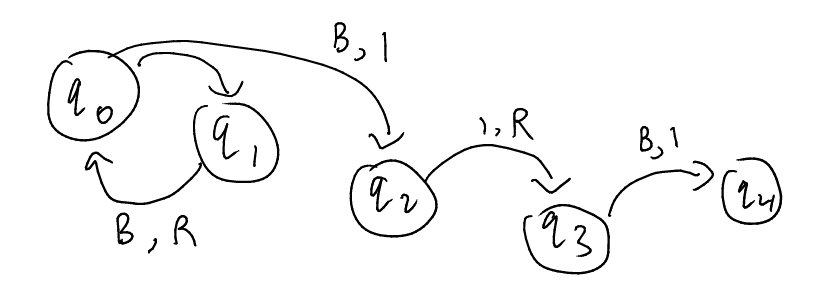
\includegraphics[width=.9\linewidth]{./Images/i27.png}
\end{center}
\end{itemize}
\end{itemize}
\item TM4: \(f(x)=x+2\)
\begin{itemize}
\item Skip all \(1\)'s and then add \(2 1\)'s
\item Alternatively, just go left and add \(2 1\)'s
\end{itemize}
\item TM5: \(f(x,y) = x+y\)
\begin{itemize}
\item Sequence of \(1\)'s and then a blank and then another sequence of \(1\)'s
\begin{itemize}
\item Delete first \(1\) and then go right until you see a blank and then write a \(1\) there
\item Need to know conventions about number of blanks in between
\end{itemize}
\end{itemize}
\item TM6: \(f(x,y)=x\cdot y\)
\begin{itemize}
\item Have to copy \(y x\) amount of times after \(y\) and then delete \(y\), more complicated, but a good exercise
\end{itemize}
\end{itemize}
How many functions are there from \(\mathbb{N} \to \mathbb{N}\)? Uncountably infinite. How many turing machines are there? Countably infinite. Why? Because there are finitely many instructions with a finite amount of states in your turing machine.
\begin{itemize}
\item This means that not every function can be represented as a turing machine, i.e. some are not computable.
\end{itemize}
\subsection{The Halting Problem}
\label{sec:org62362c6}
We can enumerate all Turing Machines based off a fixed alphabet. So we can write: \(T_1, T_2, T_3, \ldots, T_n, \ldots\).
\begin{itemize}
\item \(T_n(m): T_n\) on input \(m\)
\item \(K=\{x\in\mathbb{N}|T_x(x)\text{ halts}\}\)
\begin{itemize}
\item TMs can either halt (stop) or go on forever.
\end{itemize}
\end{itemize}
The Halting Problem is as follows: Is there a TM that decides whether \(y\in K\) or \(y \notin K\)? In other words:
\begin{equation*}
TM_k (y) =
\begin{cases}
1 & \text{if }y\in k
\\ 0 & \text{if }y \notin k
\end{cases}
\end{equation*}
\subsubsection{Claim}
\label{sec:org5dec85a}
This function is not computable. Then by Church-Turing thesis, a computer cannot compute this.

Note that \(K\) is r.e.
\begin{itemize}
\item Make a table with \(T_1\) on input \(1\), \(T_2\) on input \(2\), \ldots
\item Check at each step if it's still running or halts, to see if they eventually halt
\item Go through this table diagonally like was done for the rational numbers. This way we can list all elements of \(K\).
\end{itemize}

\subsubsection{Proof (by contradiction)}
\label{sec:org063b0a0}
Assume \(T_H\) decides the set \(K\). i.e.
\begin{equation*}
T_H (x) =
\begin{cases}
1 & \text{if }x\in k, \text{ }T_x(x) \text{ halts}
\\ 0 & \text{if }x \notin k, \text{ }T_x(x) \text{ loops}
\end{cases}
\end{equation*}
Now define a new machine:
\begin{equation*}
T_G (x) =
\begin{cases}
0 & \text{if }T_H(x)=0
\\ \text{loops} & \text{if }T_X(x)=1
\end{cases}
\end{equation*}

So \(T_G(x)=T_n(x)\) for some \(n\) (since we enumerated all Turing machines).

Want to know output of \(T_G(n)\)
\begin{itemize}
\item So machine can either give \(0\) or loop
\item It is \(0\) if \(T_H(n)=0\), i.e. \(n\notin k\) and \(T_n(n)\) loops, so \(T_G(n)\) loops. Can't loop and give \(0\) at the same time! \lightning
\item Loops if \(T_H(n)\) halts, i.e. \(n \in k\) \(T_n(n)\) halts, \(T_G(n)\) halts. Can't loop and halt! \lightning
\end{itemize}

This is diagonalization!
\section{Lecture 19 \textit{<2017-11-09 Thu>}}
\label{sec:org076d462}
\subsection{Reminder: Turing Machines \& Computers}
\label{sec:orgf652e3f}
\begin{center}
\begin{tabular}{ll}
TM & Computer\\
\hline
tape & memory/disc\\
head & processor/pointers\\
instructions & program\\
\(\square\) (square) & 1 bit\\
\end{tabular}
\end{center}
Everything you can do on a computer you can do on a Turing Machine. Things you can't do on a Turing Machine you cannot do on a computer, i.e. The Halting Problem

Turing Machines were supposed to be a formalization of "computability"
\begin{itemize}
\item Another way of analyzing computability is with functions
\begin{itemize}
\item Primitive recursive functions, which we'll try and extend to other functions
\end{itemize}
\end{itemize}
\subsection{Class of functions}
\label{sec:orgdb82668}

Inductive def of a class of functions: \(\mathbb{N}\to \mathbb{N}\)

Primitive Recursive Functions
\begin{enumerate}
\item \(z(x)=0\) (zero function)
\begin{itemize}
\item \(s(x)=\) the next number in the sequence following \(\mathbb{N}\) (successor)
\item \(P_k^i(\underbrace{x_1,\ldots,x_k}_{\vec{x}})=x_i, 1\leq i \leq k\) (projection)
\end{itemize}
\item Composition: Given \(g\) with \(m\) arguments and \(h_1,\ldots,h_m\) with \(\underbrace{k \text{ arguments}}_{\vec{x}}\)
\begin{itemize}
\item \(f(\vec{x})=g(h_1(\vec{x},\ldots,h_m(\vec{x}))\)
\item Schema of prim. rec. (\(h\) is primitive recursive)
\begin{itemize}
\item \(f(0)=d\)
\item \(f(n+1)=h(f(n),n)\)
\end{itemize}
\item Generalizing: \(g,h\) are prim. rec.
\begin{itemize}
\item \(f(0, \vec{x})=g(\vec{x})\)
\item \(f(n+1, \vec{x})=h(f(n,\vec{x}),n,\vec{x})\)
\end{itemize}
\end{itemize}
\end{enumerate}

\noindent\rule{\textwidth}{0.5pt}
\subsubsection{E.g}
\label{sec:org3ace0b8}
\begin{enumerate}
\item \(id(x) = x =P_1^1 (x)\)
\item \(plus(0,x)=x\)
\begin{itemize}
\item \(plus (n+1,x)=S(plus(n,x))\)
\item \(\implies g(x)=p_1^1(x))\)
\begin{itemize}
\item \(h(u,v,w)=S(P_3^1(u,v,w))\)
\item \(u\) is \(plus(n,x)\) , \(v=n, w=x\)
\end{itemize}
\end{itemize}
\item \(mult(x,y)\), factorial, exponentiation
\item \(pred(0)=0, pred(n+1)=n\) (only need the simple scheme, not the generalized one)
\begin{itemize}
\item \(h(u,v)=P_2^2(u,v)\)
\end{itemize}
\item 
\end{enumerate}
\begin{equation*}
cond(x,y,z) = 
\begin{cases}
y & \text{if }z=0
\\x & \text{otherwise}
\end{cases}
\end{equation*}
\begin{enumerate}
\item For relation \(R(\vec{x})\): (Characteristic function)
\end{enumerate}
\begin{equation*}
C_R(x) = 
\begin{cases}
1 & \text{if }R(\vec{x})
\\ 0 & \text{otherwise}
\end{cases}
\end{equation*}
\begin{enumerate}
\item Def by cases:
\end{enumerate}
\begin{equation*}
f(x)=
\begin{cases}
h_1(x) & \text{if }x \text{ satifies }A_1
\\ \ldots
\\ h_n(x) & \text{if }x \text{ satisfies }A_n
\end{cases}
\end{equation*}
$$f(x)=(h_1(x)\cdot C_{A_1}(x))+\ldots+(h_n(x)\cdot C_{A_n}(x))$$
Assuming they're disjoint, only one will happen at a time, i.e. you get one of these values (as that's the only one satisfied).
\begin{enumerate}
\item Bounded minimization:
\end{enumerate}
$$f(\vec{x})=\min y\leq n[h(\vec{x},y)=0]$$
\begin{itemize}
\item Tries out all \(y\)'s from \(0\) to \(n\) and as soon as \(h\) is \(0\), it will return \(y\)
\item e.g. \(h(3,0)=7\)
\begin{itemize}
\item \(h(3,1)=4\)
\item \(h(3,2)=0\)
\item With \(n=10\), \(f(3)=2\)
\item If condition is not met (none of the values up to \(n\) are \(0\), then it will return \(n\))
\end{itemize}
\item Essentially this is like searching, like a for-loop
\end{itemize}

\noindent\rule{\textwidth}{0.5pt}
Are all computable functions primitive recursion functions
\begin{itemize}
\item All primitive recursion functions can be enumerated (since they're theorems of a formal system)
\end{itemize}
Prim. rec: \(f_1,f_2,f_3,f_4,\ldots\)
\begin{center}
\begin{tabular}{lllll}
 & 1 & 2 & 3 & \ldots\\
\hline
\(f_1\) & \(f_1(1)\) & \(f_1(2)\) & \(f_1(3)\) & \\
\(f_2\) & \(f_2(1)\) & \(f_2(2)\) &  & \\
\(f_3\) & \ldots &  &  & \\
\end{tabular}
\end{center}
Let \(g(x)=f_x(x)+1\). If \(g\) were primitive recursive, then \(g(x)=f_n(x)\) for some \(n\).

So what is \(g(n)\)? \(g(n)=f_n(n)\) but by definition of \(g\), \(g(n)=f_n(n)+1\). A function cannot be the same value as a function and that function plus \(1\). \lightning

Therefore, \(g\) is \uline{not} primitive recursive. 

Primitive recursive functions are really nice and most if not all we've seen in our lives are primitive recursive.
\subsection{Bloop-Programs}
\label{sec:org4244a94}
Bloop -> Bounded loop. This is the definition used in GEB instead of defining primitive recursive functions like we just did
\subsubsection{Ex}
\label{sec:org3d7c1cb}
\begin{itemize}
\item LOOP 4 TIMES
\item BLOCK: BEGIN
\item \ldots
\item BLOCK: END
\end{itemize}
\href{http://www.cs.mcgill.ca/\~cs230/TisLoopy/index.html}{TisLoopy} from course webpage to compile Bloop-Programs and practice without having to define a primitive recursive function.
\subsubsection{Syntax}
\label{sec:org261b287}
\begin{verbatim}
DEFINE PROCEDURE "MINUS" [M,N]:
BLOCK 0: BEGIN
      OUTPUT <= 0;
      IF M<N, THEN: QUIT BLOCK 0;
      LOOP AT MOST M+1 TIMES:
      BLOCK 1: BEGIN
      	    IF OUTPUT+N=M, THEN ABORT LOOP 1;
	    OUTPUT <= OUTPUT + 1
      BLOCK 1: END
BLOCK 0: END
\end{verbatim}
\begin{center}
\begin{tabular}{rrr}
M & N & OUTPUT\\
\hline
5 & 2 & 0\\
 &  & 1\\
 &  & 2\\
 &  & 3\\
\end{tabular}
\end{center}
\section{Lecture 20 \textit{<2017-11-14 Tue>}}
\label{sec:org926cfa0}
\subsection{Bloop}
\label{sec:org054a6a8}
Bloop = primitive recursive functions. What makes them nice?
\begin{itemize}
\item Computable
\begin{itemize}
\item Note that, as seen in last class, not all computable functions are primitive recursive functions
\end{itemize}
\item Evaluation always terminates
\item Total, defined on all inputs
\end{itemize}
Big picture: \begin{center}
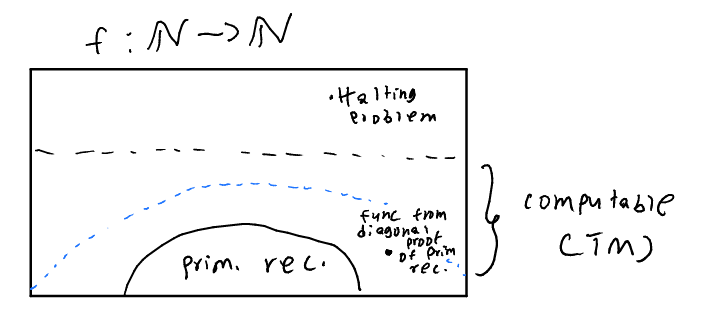
\includegraphics[width=.9\linewidth]{./Images/i28.png}
\end{center}
\begin{itemize}
\item Want to expand our definition of primitive recursive functions. How?
\end{itemize}
Recall that bloop has loops as follows: 
\begin{itemize}
\item \texttt{LOOP ... TIMES}
\item \texttt{LOOP AT MOST ... TIMES}
\item Both of the loop iterations are bounded.
\end{itemize}
\subsection{Floop}
\label{sec:org3fbbe7e}
Like Bloop but have a new block:

MU-LOOP:
\begin{verbatim}
MU-LOOP:
BLOCK:BEGIN
	ABORT LOOP
BLOCK:END
\end{verbatim}
Then we get programs, such that some terminate and some do not terminate (loop forever).

\subsection{Bounded minimization}
\label{sec:org822b781}
\(f(x) = \min y \leq n \overbrace{[h(x,y)=0]}^{\text{condition}}\)
\begin{itemize}
\item How to compute?
\item Start with \(y=0\), keep evaluating and iterating until it's \(0\) (then you output \(y\)) or you reach the end and you output the end \((n)\).
\end{itemize}

\begin{equation*}
prime(x) = 
\begin{cases}
1 & \text{if }x \text{ is prime}
\\ 0 & \text{otherwise}
\end{cases}
\end{equation*}

E.g. \(nextprime(x)\min y \leq (x! + 1)[x < y \text{ AND }prime(y)=1]\)
\begin{itemize}
\item \(listprimes(0)=2\)
\item \(listprimes(n+1)=nextprime(listprimes(n))\)
\end{itemize}
\subsection{Unbounded minimization}
\label{sec:org041bd20}
\(f(x)=\) the least \(y\), such that \(\overbrace{y+x=5}^{\text{condition}}\)
\begin{center}
\begin{tabular}{llllllll}
\(x:\) & \(0\) & \(1\) & \(2\) & \(3\) & \(4\) & \(5\) & \(6\)\\
\(f(x):\) & \(5\) & \(4\) & \(3\) & \(2\) & \(1\) & \(0\) & undefined \(\uparrow\)\\
\end{tabular}
\end{center}
(\(\uparrow\) means undefined)

This is called the \(\mu-\text{operator}\) (least search operator):
\begin{itemize}
\item \(\mu y [f(\vec{x},y)=0] \implies z\) iff \(f(\vec{x},z)=0\) and for every \(y<z, f(\vec{x},y)\) \uline{is defined} (and \(> 0\))
\end{itemize}

E.g. \(\mu y [f_i(y)=0]\)
\begin{center}
\begin{tabular}{lllllllll}
\(x\) & \(0\) & \(1\) & \(2\) & \(3\) & \(4\) & \(5\) & \(6\) & \ldots\\
\(f_1(x)\) & \(3\) & \(2\) & \(1\) & \(0\) & \(0\) & \(0\) & \(0\) & \ldots\\
\(f_2(x)\) & \(2\) & \(0\) & \(\uparrow\) & \(3\) & \(\uparrow\) & \(0\) & \(0\) & \ldots\\
\(f_3(x)\) & \(2\) & \(3\) & \(\uparrow\) & \(1\) & \(0\) & \(\uparrow\) & \ldots & \\
\end{tabular}
\end{center}
\begin{itemize}
\item \(\mu y [f_1(y)=0] \implies 3\)
\begin{itemize}
\item Because \(f_1(3)\) is the first to be \(0\) and the previous values are defined.
\end{itemize}
\item \(\mu y [f_2(y)=0] \implies 1\)
\item \(\mu y [f_3(y)=0] \implies \uparrow\)
\begin{itemize}
\item It is undefined because not all \(f_3(y)\) are defined before \(f_3(z)=0\)
\end{itemize}
\end{itemize}

Can we make a Turing Machine that acts like this \(\mu\) operator?
\begin{itemize}
\item Yes. The Turing Machine goes through a row until it either hits \(0\) or \(\uparrow\) (loops forever)
\begin{itemize}
\item Note that we can't determine in finite time if something loops forever
\end{itemize}
\item Recall that Turing Machines can loop forever, which may happen if a function keeps evaluating to something that isn't \(0\) but is defined.
\item \(\implies\) computable
\item \(f(x) \uparrow \iff\) TM loops forever
\end{itemize}
\subsection{Partial recursive functions}
\label{sec:org8d509c8}
\begin{itemize}
\item Primitive recursive functions
\item \(\mu-\text{operator}\)
\end{itemize}

Some partial rec. fun. are defined (has a value) for \uline{all} arguments: total functions (so we can distinguish between partial rec. fun and total partial rec. fun)
\begin{itemize}
\item We call these recursive functions
\end{itemize}
\begin{center}
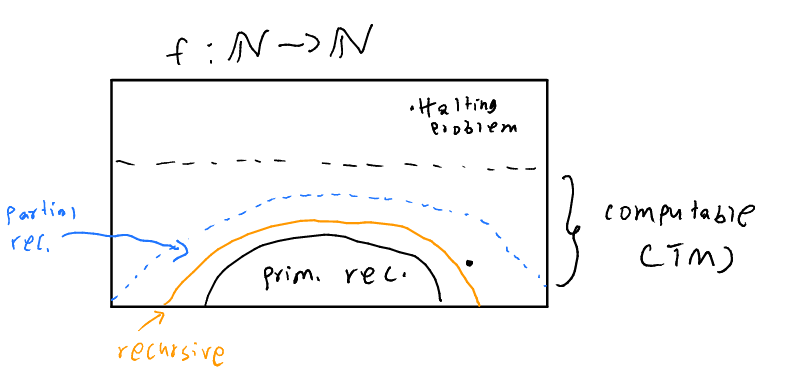
\includegraphics[width=.9\linewidth]{./Images/i29.png}
\end{center}

Alternatively: 
\begin{tabular}{l l | l}
prim. rec | rec. & not total part. rec
\\ \hline total & not total
\end{tabular}
Are primitive functions syntactic or semantic? Syntactic. The definition is typographical. Partial rec. functions are also syntactic.
\begin{itemize}
\item But recursive functions are semantic because you can't just look at a function and determine if its recursive. It needs to be defined, needs a meaning.
\end{itemize}

\noindent\rule{\textwidth}{0.5pt}
How did we show that there was a computable function that wasn't primitive recursive? Diagonalization. Can you use diagonalization to create a computable function that isn't partial recursive.
\begin{center}
\begin{tabular}{lllll}
 & \(0\) & \(1\) & \(2\) & \(3\)\\
\hline
\(\varphi_0\) & \(\varphi_0(0)\) & \(\varphi_0(1)\) & \(\varphi_0(2)\) & \(\varphi_0(3)\)\\
\(\varphi_1\) & \(\varphi_1(0)\) & \(\varphi_1(1)\) & \ldots & \\
\(\varphi_2\) & \ldots &  &  & \\
\end{tabular}
\end{center}

Define: \(\psi_1(x)=\underbrace{\varphi_x(x)}_{\text{might be undefined}}+1\)
\begin{equation*}
\psi_2(x) = 
\begin{cases}
1 & \text{if }\varphi_x(x) \uparrow
\\ 0 & \text{if }\varphi_x(x) \downarrow
\end{cases}
\end{equation*} 

The Halting Problem for partial recursive functions is \uline{not} recursive: There is no recursive function that tells us whether \(varphi_x(x)\) is defined or not. Assume:
\begin{equation*}
f(x) \simeq 
\begin{cases}
1 & \text{if } \varphi_x(x) \downarrow
\\ 0 & \text{if }\varphi_x(x) \uparrow
\end{cases}
\end{equation*}
is a total partial rec. function
\begin{itemize}
\item (this is recursive, since \(f(x)\) always gives you a value).
\end{itemize}
Define
\begin{equation*}
p(x) \simeq 
\begin{cases}
\uparrow & \text{if } f(x)=1
\\ 0 & \text{if }f(x)=0
\end{cases}
\end{equation*}
\(p(x)=\mu y [y+f(x)=0]\)
\begin{itemize}
\item Then \(p(x)\) is partial recursive because it's just the \(\mu-\text{operator}\) applied on another partial recursive function.
\end{itemize}
Because \(p(x)\) is partial recursive, it must occur in the enumeration such that \(p(x)=\varphi_y(x)\)
\begin{itemize}
\item What is \(p(y)\)? \(p(y)=\varphi_y(y)\). It is undefined if \(f(y)=1\) and \(f(y)=1\) if \(\varphi_y(y)\) is defined. Contradiction (\(p(y)\) is defined and undefined at the same time). \lightning
\end{itemize}
\section{Lecture 21 \textit{<2017-11-16 Thu>}}
\label{sec:org6e04196}
Review of Turing Machines
\subsection{Turing Machine on Handout 5}
\label{sec:orgd05adb3}
This machine doubles a string of \(1\)'s
\begin{itemize}
\item Doubling 1: \begin{center}
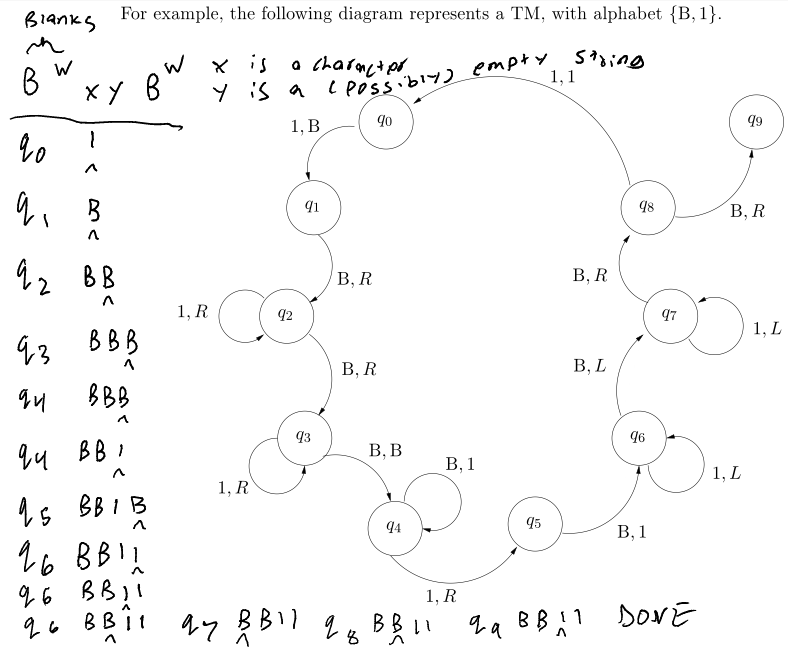
\includegraphics[width=.9\linewidth]{./Images/i30.png}
\end{center}
\item Doubling 3 (part of execution): \begin{center}
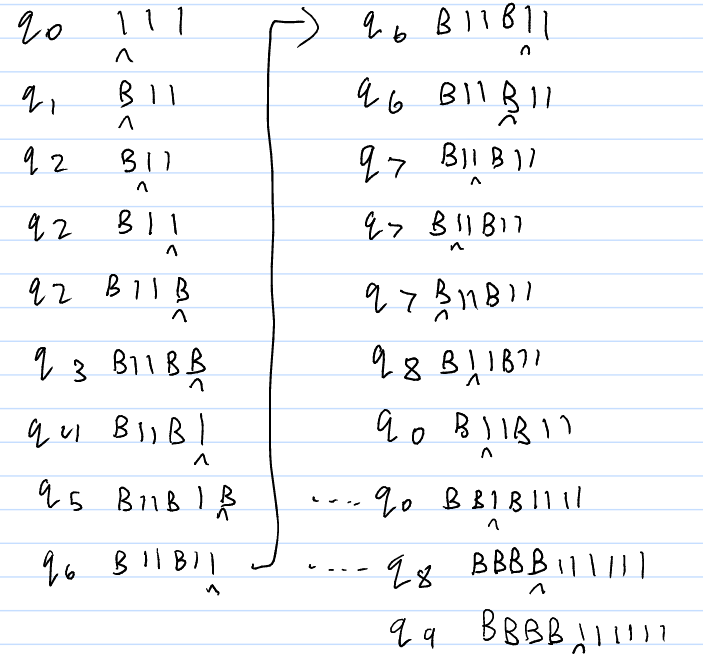
\includegraphics[width=.9\linewidth]{./Images/i31.png}
\end{center}
\end{itemize}
\subsection{Turing Machine for addition}
\label{sec:org2097755}
\begin{center}
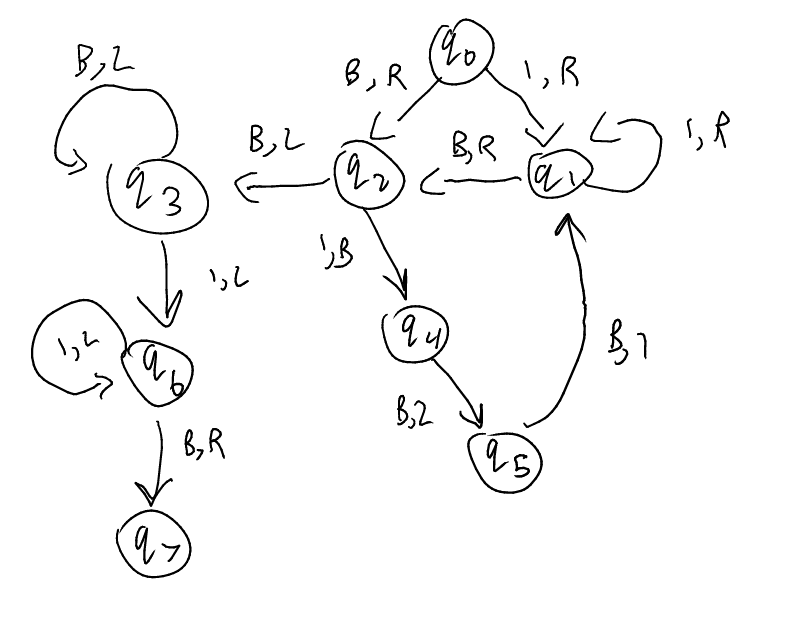
\includegraphics[width=.9\linewidth]{./Images/i32.png}
\end{center}

\begin{center}
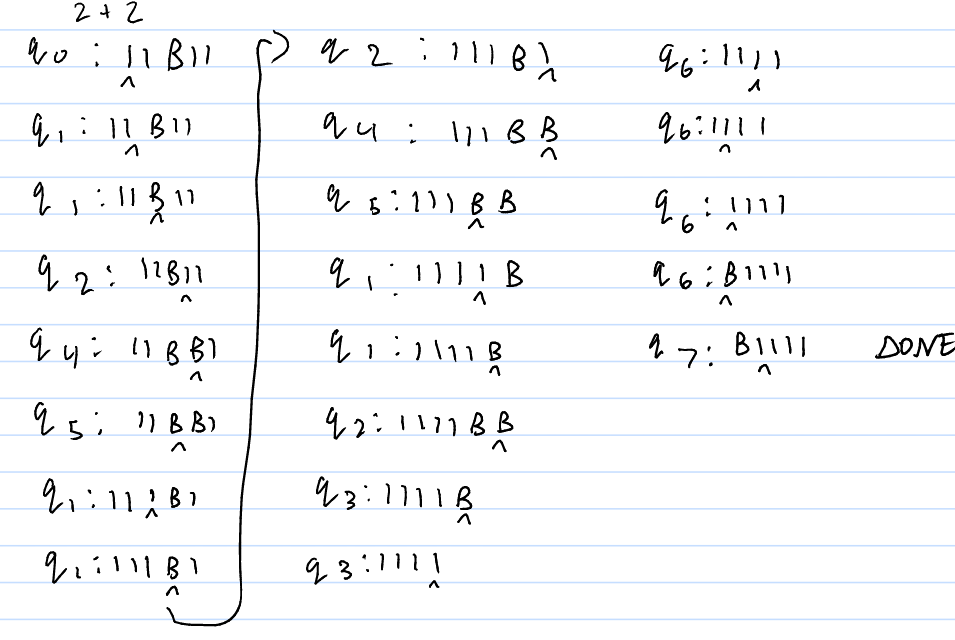
\includegraphics[width=.9\linewidth]{./Images/i33.png}
\end{center}

Try: \url{http://turingmachinesimulator.com/shared/tsgfopdqwb}

\subsection{Turing Machine for multiplication}
\label{sec:org2f5dd62}
We're not actually going to make one, but what if we wanted to? We would reuse our Turing Machine for addition, don't reinvent the wheel from scratch each time. Note that:
\begin{equation*}
n \times m = 
\begin{cases}
0 & \text{if }n=0
\\ (n-1) \times m + m & \text{if }n>0
\end{cases}
\end{equation*}
Can recursively add in order to multiply. 

\subsection{The Halting Problem}
\label{sec:org9bb27c2}
This helps you understand the Halting Problem more. \begin{center}
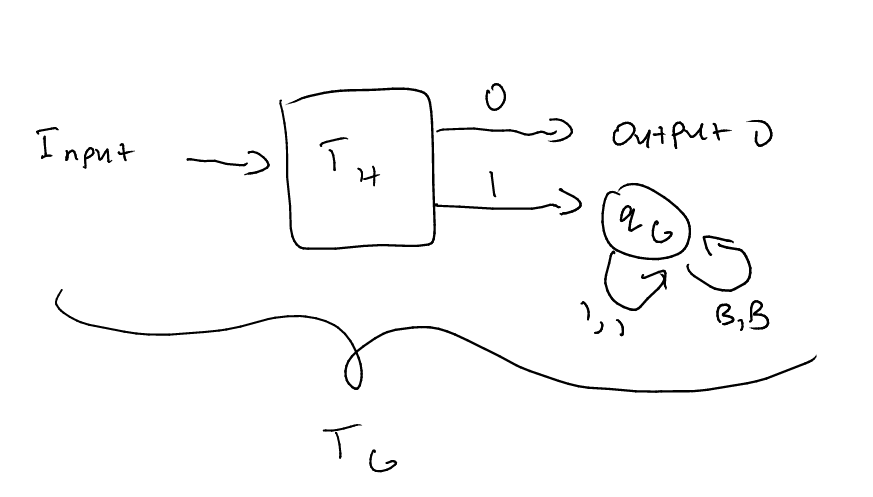
\includegraphics[width=.9\linewidth]{./Images/i34.png}
\end{center}
\begin{itemize}
\item Turing Machines can be inputted as an argument for another
\item Review of Halting Problem
\item Key points:
\begin{itemize}
\item Assuming existence of \(T_H\)
\item Constructing the \(T_G\) through elementary operations on \(T_H\)
\item Self-reference (feeding \(T_G\) to itself)-> \lightning
\end{itemize}
\end{itemize}
\section{Lecture 22 \textit{<2017-11-21 Tue>}}
\label{sec:orgcfed8db}
\subsection{Quiz Review}
\label{sec:org2ce64f1}
\begin{itemize}
\item Non logical symbols in FOA: \(0, S, +, \times\)
\item Halting set: \(K=\{n\in \mathbb{N} | T_n(n) \text{ halts}\}\)
\item Partial recursive def
\item \(\mu y [S(y) \text{ op }1 = 0]\)
\begin{itemize}
\item \(f(1)=0, f(0)=\uparrow\)
\end{itemize}
\item \(\aleph_0\) Turing Machines/Primitive Recursive Functions
\end{itemize}
\subsection{Functions}
\label{sec:orgd508e6d}
\begin{center}
\begin{tabular}{lll}
Prim. rec & BlooP & -\\
Part. rec & FlooP & TM\\
Rec. & terminating FlooP & TM always halt\\
\end{tabular}
\end{center}
\subsection{Representability}
\label{sec:org19516c7}
\begin{center}
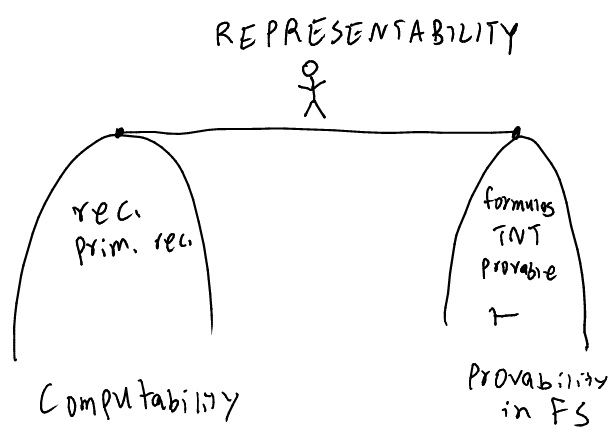
\includegraphics[width=.9\linewidth]{./Images/i35.png}
\end{center}
Today we will learn how to go from computability to provability in a formal system.

A predicate is \uline{represented} in a FS:
\begin{enumerate}
\item All true instances are theorems in FS
\item All false instances are not thms
\end{enumerate}

\subsubsection{Ex.}
\label{sec:org6de6fa3}
\uline{Express}: Evenness
\begin{equation*}
Even(x) = 
\begin{cases}
1 & \text{if }\exists y: x=2\cdot y
\\ 0 & \text{otherwise}
\end{cases}
\end{equation*}
Represented in TNT: 
\begin{itemize}
\item \(TNT \vdash Even(SS0)\)
\item \(TNT \nvdash Even(S0)\)
\item \(TNT \vdash \sim Even(S0)\)
\end{itemize}
\subsubsection{Thm}
\label{sec:org32d2f4e}
Any primitive recursive predicate (BlooP) is representable in FOA.
\begin{itemize}
\item Recall: What is a primitive recursive predicate? A predicate is primitive recursive if its characteristic function is primitive recursive
\item \(Even(x) = \forall x : \exists y : \ldots\)
\end{itemize}
\subsubsection{Thm}
\label{sec:org932f74a}
Any recursive predicate is representable in FOA
\subsection{Theories of Arithmetic}
\label{sec:org835aec0}
(Handout 8)
\begin{center}
\begin{tabular}{llll}
\(\Pi_0\text{/baby}\) & \(\Pi_1\text{/junior}\) & \(\Pi_2\text{/Q}\) & \(\Pi\text{/FOA}\)\\
4 axiom schemas & 4+3 axiom schemas & finitely many (9) axioms & 4 schema + induction\\
\end{tabular}
\end{center}
\(\Pi_0 \nvdash 0 \neq S0\)

$$\Pi_0 \subset \Pi_1 \subset \Pi_2 \subset \Pi $$
\subsection{Proof-Pairs}
\label{sec:org5f0333d}
TNT-PROOF-PAIR(n,m), where \(n\) is the G$\backslash$"odel \# of a proof of \(m\) and \(m\) is the G$\backslash$"odel \# of the theorem

The property of being a proof-pair is primitive recursive (it's like proof checking, just decompose it and see if it works): proof-pair(x,y)
\begin{itemize}
\item This means that it's representable
\begin{itemize}
\item \(\implies\) There is a FOA-formula Bew(x,y) (German word Beweis = proof) that represents it.
\end{itemize}
\end{itemize}
Being a theorem-number:
\begin{itemize}
\item \(theorem-number(x) = \exists y:proof-pair(y,x)\)
\begin{itemize}
\item i.e. \(x\) is a theorem number if it's a G$\backslash$"odel number of a theorem
\item Is this primitive recursive? Not clear. You have to find a proof rather than check a proof.
\end{itemize}
\end{itemize}
\subsection{Substitutions}
\label{sec:org2598219}
\begin{center}
\begin{tabular}{ll}
Formula & G$\backslash$"odel \#\\
\(a=a\) & 262 111 262\\
\(SS0=SS0\) (substitute by term) & 123 123 666 111 123 123 666\\
\end{tabular}
\end{center}
SUB(formula with free variable, numeral (term), resulting formula) -> In our example, SUB(262 111 262, 2, 123 123 666 111 123 123 666)   
\begin{itemize}
\item This is primitive recursive
\begin{itemize}
\item This means that there is a formula in TNT that represents it
\end{itemize}
\item All we have to do to check this is just decode the first formula, plug in the numeral into it and see if it's equal to the resulting formula
\end{itemize}

SUB(x,y,z)
\begin{itemize}
\item Good exam question, which numbers represent x,y,z?
\end{itemize}

ARITHMOQUINE(a,b) = SUB(a,a,b)
\section{Lecture 23 \textit{<2017-11-23 Thu>}}
\label{sec:orgd5e9284}
What is a theory? Set of sentences closed under deduction. \(x\in T \iff T \vdash x\), where \(T\) is a theory.

A theory \(T\) is \uline{complete}, if for all sentences \(A\): either \(T \vdash A\) or \(T \vdash \sim A\)

What we will show next is that TNT is not complete (incomplete)!
\begin{itemize}
\item Proof: Produce \(G\), s.t. \(TNT \nvdash G\) and \(TNT \nvdash \sim G\)
\item This is (more or less) G$\backslash$"odel's First Incompleteness Theorem
\begin{itemize}
\item Very important, perhaps the highlight of the course
\end{itemize}
\end{itemize}
ARITHMOQUINE(a,b) = SUB(a,a,b)
\begin{itemize}
\item \(a\) is a G$\backslash$"odel number of a formula with a free variable, the second \(a\) is the number that stands for a certain numeral and \(b\) is the G$\backslash$"odel number of the formula from the first \(a\), but with the free variable replaced by the numerable represented by the second \(a\)
\end{itemize}
\subsection{Ex}
\label{sec:orgdd99f0c}
\(A(x)\) is \(\sim (Sx=0)\)
\begin{itemize}
\item We want to get the ARITHMOQUINE of this number
\item G$\backslash$"odel number is: \(a = 223 362 123 262 111 666 323\)
\item ARITHMOQUINE(a,b)
\begin{itemize}
\item Take \(A(a)\) => \(\sim (S\underbrace{SS \ldots S}_{a-many}0 = 0)\)
\begin{itemize}
\item Now take the G$\backslash$"odel number of this and you get your \(b\)
\end{itemize}
\end{itemize}
\item Arithmoquine is certainly recursive and terminates. We can easily make a computer program to mimic it.
\end{itemize}
More mathematically: Arithmoquine is usually called: d (diagonal function)

\begin{equation*}
d(\underbrace{\#\alpha}_{\text{the Godel \# of $\alpha$}} =
\begin{cases}
\#\alpha (S_{\#\alpha}) & \text{if $\#\alpha$ is the Go of a form $\alpha$ with one free variable}
\\ \#\alpha & \text{otherwise}
\end{cases}
\end{equation*}
\begin{itemize}
\item E.g. \(d(5) = 5, d(a)=b\)
\end{itemize}

\noindent\rule{\textwidth}{0.5pt}
\begin{itemize}
\item \(Even (x)\) expresses "x is even"
\item \(Even (SSSS0)\) expresses "4 is even"
\item \(A(x)\) "x has the property A"
\item \(A(SSSS0)\) "4 has the property A"
\end{itemize}

A number (ex. student id), can just be a number but it can represent a student.

IS-TNT-AXIOM(x) => property of the number \(x\) or property of the formula with G$\backslash$"odel \# x
\begin{itemize}
\item \(\forall a : \exists b: \ldots x \ldots\)
\end{itemize}

G's aunt:
\begin{itemize}
\item \(\sim \exists a : \exists a': \underbrace{TNT-PROOF-PAIR(a,a')}_{a \text{ is a proof of }a'} \wedge \underbrace{ARITHMOQUINE(a'', a')}_{a' \text{ is the arithmoquinification of }a''} = F(a'')\) with G$\backslash$"odel \# \(u\)
\begin{itemize}
\item Equation has one free variable, \(a''\)
\item Putting them together we get \(a\) is a proof of the arithmoquinification of a''
\end{itemize}
\item Now G's aunt is:
\begin{itemize}
\item there is no (\(a\), s.t. \(a\) is a) TNT proof of (\(a'\) and \(a'\) is )the arithmoquinification of a''
\end{itemize}
\end{itemize}
Now we plug in \(u\) as the free variable \(a''\)
\begin{itemize}
\item \(\sim \exists a : \exists a': TNT-PROOF-PAIR(a,a') \wedge ARITHMOQUINE (\underbrace{SS\ldots S 0}_{u \text{ many}},a') = F(u) = G\)
\item This is now a sentence, no more free variables
\end{itemize}
What is the G$\backslash$"odel \# of \(G\)? The arithmoquinification of \(u\).
\begin{itemize}
\item We have done the same thing we did earlier with the smaller example except for a longer formula.
\end{itemize}
What does \(G\) express? There is no TNT-proof of \(\underbrace{\text{the arithmoquinification of }u}_{G}\).

=> \(G\) says: "I am unprovable (in TNT)"
\begin{itemize}
\item Is G a TNT theorem? Assume TNT \(\vdash G\). Since we're working in a system that is sound, then \(G\) must be true. But \(G\) expresses that it is not a TNT theorem. \lightning
\item => TNT \(\nvdash G\)
\item Is \(\sim G\) a TNT-theorem? Assume TNT \(\vdash \sim G\). So, \(\sim G\) true, i.e. \(G\) is provable in TNT. So TNT \(\vdash G\) => TNT is inconsisten.
\item If TNT is consistent then TNT \(\nvdash \sim G\)
\end{itemize}
So we end up with: If TNT is consistent, then TNT is not complete! \textbf{G$\backslash$"odel's First Incompleteness Theorem}
\begin{itemize}
\item TNT was important here to tell us that the functions we used (i.e. TNT-PROOF-PAIR) are representable
\item We did not need TNT directly, we could have used a weaker theory, like \(\Pi_1\)
\end{itemize}
\subsection{General Version of G$\backslash$"odel's First Incompleteness Theorem}
\label{sec:orge6225f0}
\(G1\): Every theory that includes \(\Pi_1\) is consistent (or else you prove everything, including \(G\)) and axiomatizable (has an axiom system, or else we wouldn't have anywhere to start, we need to be able to define what a proof is) is incomplete.
\begin{itemize}
\item How could you make \(G\) provable in TNT?
\begin{itemize}
\item Just turn it into an axiom
\item So we can do something like TNT\(+G\)
\begin{itemize}
\item But this still includes \(\Pi_1\) and is axiomatizable (because TNT has axioms)
\item But then you can do the same thing with this new system and get something similar, say \(G'\)
\item This will once again, be incomplete
\end{itemize}
\item As long as you're axiomatizable, you'll still be incomplete, no matter how much we try to extend TNT.
\end{itemize}
\end{itemize}
\end{document}